\chapter{Delay Networks}
\label{chapt:delays}

This chapter has been adapted from, while significantly extending, the work of \citet[][patent pending]{voelker2015computing, dynamicspatent, voelker2018}.

A particularly important dynamical system that has not been discussed before in the NEF literature is the pure \emph{continuous-time delay} line.
In order to implement such a system, one must represent a \emph{rolling window} of input history, or, in other words, one must \emph{buffer} the input signal into a memory that continuously slides alongside the current input.
In this chapter, we provide a novel derivation of an optimal low-dimensional linear approximation to a continuous-time delay, and then realize this \emph{delay network} using the NEF in a recurrent spiking network.
We then investigate its computational properties, proving that the resulting network implements a well-defined nonlinear encoding of its input across the delay interval -- isomorphic to a high-dimensional projection of the Legendre polynomials.
This network uses a scale-invariant representation, with a level of accuracy that depends on the input frequency, chosen dimensionality (i.e.,~the order of the approximation), and particular synapse model.
To our knowledge, this work is the first to demonstrate that such a temporal code may be accurately implemented using a spiking dynamical network.

Reservoir Computing approaches, such as Liquid State Machines~\citep{maass2002real} and Echo State Networks~\citep{jaeger2001echo}, may be used to approximate a delay line.
However, since these networks use randomly chosen feedback weights, we show in section~\ref{sec:delay-rc} that they do so with relatively poor accuracy despite extensive hyperoptimization.
Such networks instead represent a random variety of nonlinear memory traces~\citep{lukovsevicius2012reservoir}.
Discrete approaches to short-term memory, such as those taken by \citet{white2004short} and \citet{ganguli2008memory}, while optimal in an information-theoretic sense, rely fundamentally on single time-step delays between rate-based neurons.
In contrast, the method that we propose here works independently of the simulation time-step, and is optimal assuming the population of spiking neurons---coupled with some model of the synapse---accurately represents a low-dimensional, low-frequency, vector space.
Furthermore, our framework is extended to account for arbitrary linear synapses, which improves our understanding of the relationship between synapse models and network-level computation.

We also find that the delay-line is a difficult function for FORCE networks (section~\ref{sec:force-comparison}), as re-encoding the delayed output as a teaching signal ends up ``confusing'' the network.
Furthermore, we find that our network, when expressed as an RNN cell (without spikes), outperforms equivalently-sized stacked LSTMs on computing long delays, and predicting the Mackey-Glass dataset---a difficult chaotic time-series benchmark---in training time, inference time, and test accuracy.
Next, we reveal some connections between the neural responses within our delay network, and ``time cells'' in the neuroscience literature.
Lastly, we discuss a number of theoretical applications that are directly supported by, and extend, the computations of the delay network.

Now consider a continuous-time delay line of $\theta$ seconds:
\begin{align} \label{eq:time-delay}
y(t) = (u \ast \delta_{\theta})(t) = u(t - \theta)\text{,} \quad \theta > 0 \text{,}
\end{align}
where $\delta_{\theta}$ denotes the Dirac delta shifted forwards in time by $\theta$.
This system takes a time-varying scalar signal, $u(t)$, and outputs a purely delayed version, $u(t - \theta)$.
The task of computing this function both accurately and efficiently in a biologically plausible, spiking, dynamical network, is a significant theoretical challenge, that, to our knowledge, has previously remained unsolved.

The continuous-time delay is worthy of detailed consideration for several reasons.
First, it is non-trivial to implement using continuous-time spiking dynamical primitives.
Specifically, equation~\ref{eq:time-delay} requires that we maintain a \emph{rolling window} of length $\theta$ (i.e.,~the history of $u(t)$, going $\theta$ seconds back in time).
Thus computing a delay of $\theta$ seconds is just as hard as computing every delay of length $\theta'$, for all $0 \le \theta' \le \theta$.
Since any finite interval of $\mathbb{R}$ contains an uncountably-infinite number of points, an exact solution for arbitrary $u(t)$ requires that we maintain an uncountably-infinite amount of information in memory.
Second, the delay provides us with a window of input history from which to compute arbitrary nonlinear functions across time.
For instance, the spectrogram of a signal may be computed by a nonlinear combination of delays, as may any finite impulse response~(FIR) filter.
Third, delays introduce a rich set of interesting dynamics into large-scale neural models, including: oscillatory bumps, traveling waves, lurching waves, standing waves, aperiodic regimes, and regimes of multistability~\citep{roxin2005role}.
Fourth, a delay line can be coupled with a single nonlinearity to construct a network displaying many of the same benefits as Reservoir Computing~\citep{appeltant2011information, bai2018dfr}.

Many learning algorithms also tend to rely on sliding windows of input history.
For instance, \citet{leng2013online} and \citet{izzeldin2011online} improved their neural networks' accuracy by incorporating sliding windows into their learning rules -- but they did not offer any neural implementation for the component that performs the required buffering.
Similarly, \citet{ferreira2009online} found sliding windows to be beneficial for the online learning of process models, in which the parameters of a nonlinear time-varying system are identified.

The computational power of delays is explained much more broadly by Takens' embedding theorem~\citep{takens1981detecting, noakes1991takens}.\footnote{%
We thank Peter Suma for pointing out this connection.
}
This theorem provides a very deep connection between delays and dynamical systems, specifically: any chaotic attractor, with finite box counting dimension, $k$, can be reconstructed by a static nonlinear projection of $2k$ different delays of just \emph{one} of its internal state variables.
In other words, a basis of delays, when applied to just a single observed variable, provides enough information to infer its entire unobserved state.
These insights have practical applications to time-series forecasting in the natural sciences~\citep{sugihara2012detecting}.
And in particular, this provides theoretical grounding for why delays might be computationally useful in biological systems; their dynamics support the inference of high-dimensional states from low-dimensional observations over time.

Our delay network is also somewhat analogous to an autoencoder~\citep{gulli2017deep} from machine learning.
However, rather than compressing the input into a low-dimensional space that allows for it to be reconstructed spatially, we do this \emph{temporally}.
This leads to a number of applications that can, in effect, mentally travel back in time using just a handful of latent state-variables embedded within a spiking network.
The resulting representations are fully interoperable with the semantic pointer architecture~\citep[SPA;][]{eliasmith2012}, and thus afford the same manipulations as semantic pointers in Spaun, namely: binding into working memory, compressing information from cortex, internally routing information, and driving motor actions~\citep{eliasmith2013build}.

At a higher level, any physical realization of a delay must necessarilly be modelling the statistics of its input in some way.
This is because it is physically impossible to buffer arbitrary signals in continuous time (details in section~\ref{sec:nef-delay}), and thus some sacrifice must be made.
In essence, this sacrifice amounts to a sparse coding mechanism, in which a low-dimensional representation is constructed that maps onto the infinite-dimensional time window~\citep{blumensath2009sampling}.
Spikes in a neural network are akin to such a compression mechanism in time, as are decoders in space.
Our solution leverages both methods of sparsification, but not in a way that one might come to expect from information theory or other approaches involving discrete samples; our NEF-based approach finds the optimal system for linearly mapping continuous-time windows onto a low-dimensional manifold.

\section{Derivations}

It is impossible in practice (i.e.,~given finite-order continuous-time resources) to implement an arbitrary delay.
For instance, a white noise signal contains an uncountably-infinite amount of information within any finite window, that cannot be compressed any further~\citep{cover2012elements}.
We instead approximate $u(t)$ as a low-frequency signal, or, equivalently, approximate equation~\ref{eq:time-delay} as a low-dimensional system expanded about the zeroth frequency in the \emph{Laplace domain}.
Our choice of a zero-frequency approximation is informed by our analysis from section~\ref{sec:energy-minimization}, which suggests that neural systems require energy that grows linearly in the representational frequency.

\subsection{Optimal approximation}
\label{sec:nef-delay}

% However, different approximations at this stage would allow for more efficient coding of particular statistics.
We begin by transforming equation~\ref{eq:time-delay} into the Laplace domain, $\mathcal{L} \left\{ y(t) \right\} = \mathcal{L} \left\{ u(t) \right\} \mathcal{L} \left\{ \delta_{\theta}(t) \right\}$, and then using the fact that $\mathcal{L} \left\{ \delta_{\theta}(t) \right\} = e^{-\theta s}$ to obtain:
\begin{align} \label{eq:tf-delay}
F(s) := \frac{\mathcal{L} \left\{ y(t) \right\}}{\mathcal{L} \left\{ u(t) \right\}} = e^{-\theta s} \text{,}
\end{align}
where $F(s)$ is known as the \emph{transfer function} of the system, defined as the ratio of the Laplace transform of the output to the Laplace transform of the input.
Equation~\ref{eq:tf-delay} should be understood as an equivalent way of expressing equation~\ref{eq:time-delay} in the Laplace domain, where the variable $s$ denotes a complex frequency. 
Notably, we have not made any sacrifices at this point, as the ideal system is a linear dynamical system.
Thus far, we have only described the transfer function that we would like the network to implement. %while $t$ is non-negative in the time domain.
% Unimportant reminder? The transfer function is the Laplace transform of system's impulse response.

The state-space model discussed in section~\ref{sec:principle3} (equation~\ref{eq:lti}) is related to its transfer function by equation~\ref{eq:ss2tf}.
Conversely, a transfer function can be converted into a state-space model satisfying equation~\ref{eq:ss2tf} \emph{if and only if} it can be written as a proper ratio of finite polynomials in $s$~\citep{brogan1982modern}.
The ratio is proper when the degree of the numerator does not exceed that of the denominator.
In such a case, the output will not depend on future input, and so the system is \emph{causal}.
The degree of the denominator corresponds to the dimensionality of the state-vector, and therefore must be finite.
These two conditions align with physically realistic constraints where time may only progress forward, and neural resources are limited.

However, the pure delay (equation~\ref{eq:tf-delay}) has infinite order when expressed as a ratio of polynomials in $s$, and so the system is irrational, or infinite-dimensional.
Consequently, no finite state-space model will exist for $F(s)$, which formalizes our previous remark that an exact solution is impossible for finite, continuous-time systems.
To overcome this, we must approximate the irrational transfer function $e^{-\theta s}$ as a proper ratio of finite-order polynomials.
We do so using its \emph{Pad\'e approximants}---the coefficients of a Taylor series extended to the ratio of two polynomials---expanded about $s=0$~\citep{Pade1892, vajta2000some}:
\begin{equation} \label{eq:pade}
\begin{aligned}
\left[ p/q \right] e^{-\theta s} &= \frac{\mathcal{B}_{p}(-\theta s)}{\mathcal{B}_{q}(\theta s)} \text{,} \\
\quad \mathcal{B}_m(s) &:= \sum_{i=0}^m \begin{pmatrix}m \\ i\end{pmatrix} \frac{(p + q - i)!}{(p + q)!} s^i \text{.}
\end{aligned}
\end{equation}
This provides the transfer function of order $p$ in the numerator and order $q$ in the denominator that optimally approximates equation~\ref{eq:tf-delay} for low-frequency inputs (i.e.,~up to order $p + q$).

After choosing $0 \le p \le q$, we may numerically find a state-space model $(A\text{,}\, B\text{,}\, C\text{,}\, D)$ that satisfies equation~\ref{eq:ss2tf} using standard methods,\footnote{%
For instance, the function \texttt{tf2ss} in MATLAB or SciPy.}
and then map this system onto the synapse using Principle~3.
%This works independently of the chosen simulation time-step using equation~\ref{eq:p3discrete}.
However, na\"ively applying this conversion leads to numerical issues in the representation (i.e.,~dimensions that grow exponentially in magnitude), due in part to the factorials in equation~\ref{eq:pade}.

To overcome this problem, we derive an equivalent yet normalized state-space model that we have not encountered elsewhere.
We do so for the case of $p = q - 1$, since this provides the best approximation to the step-response. We symbolically transform equation~\ref{eq:pade} into a normalized state-space model that avoids the need to compute any factorials.
We first do so for the special case of $p = q - 1$, since this provides the best approximation to the step-response~\citep{vajta2000some}.
We begin by expanding equation~\ref{eq:pade}:
\begin{align*}
[q-1/q]e^{-\theta s} &= \frac{\sum_{i=0}^{q-1} \begin{pmatrix}{q-1} \\ i\end{pmatrix} (2q - 1 - i)! (-1)^i \theta^i s^i}{\sum_{i=0}^q \begin{pmatrix}q \\ i\end{pmatrix} (2q - 1 - i)! \theta^i s^i} \\
&= \frac{\frac{1}{\theta^{q} (q-1)!} \sum_{i=0}^{q-1} \frac{(q-1)!}{(q-1-i)!i!} (2q - 1- i)! \theta^i s^i (-1)^i}{s^q + \frac{1}{\theta^q (q-1)!}  \sum_{i=0}^{q-1} \frac{q!}{(q-i)!i!} (2q - 1 - i)! \theta^i s^i} \\
&= \frac{\sum_{i=0}^{q-1} c_i s^i}{s^q + \sum_{i=0}^{q-1} d_i s^i} \text{,}
\end{align*}
where $d_i := \frac{q(2q - 1 - i)!}{(q-i)!i!} \theta^{i-q}$ and $c_i := (-1)^i \left( \frac{q-i}{q} \right) d_i$.

This transfer function is readily converted into a state-space model in controllable canonical form:
\begin{equation*}
    \begin{alignedat}{2}
        A &= \begin{pmatrix} -d_{q-1} & -d_{q-2} & \cdots & -d_0 \\ 1 & 0 & \cdots & 0 \\ 0 & \ddots & \ddots & \vdots \\ 0 & 0 & 1 & 0\end{pmatrix} \text{,} & & \quad\quad \begin{alignedat}{1}
            B &= \transpose{\begin{pmatrix} 1 & 0 & \cdots & 0\end{pmatrix}} \text{,} \\
            C &= \begin{pmatrix} c_{q-1} & c_{q-2} & \cdots & c_0\end{pmatrix} \text{,} \\
            D &= 0 \text{.}
        \end{alignedat}
    \end{alignedat}
\end{equation*}
To eliminate the factorials in $d_i$ and $c_i$, we scale the $i^{\text{th}}$ dimension of the state-vector by $d_{q-1-i}$, for all $i = 0 \ldots q - 1$.
This is achieved without changing the transfer function by scaling each $(B)_j$ by $d_{q-1-j}$, each $(C)_i$ by $1 / d_{q-1-i}$, and each $(A)_{ij}$ by $d_{q-1-i} / d_{q-1-j}$, which yields the equivalent state-space model:
\begin{equation}
    \begin{alignedat}{2}
        A &= \begin{pmatrix} -v_0 & -v_0 & \cdots & -v_0 \\ v_1 & 0 & \cdots & 0 \\ 0 & \ddots & \ddots & \vdots \\ 0 & 0 & v_{q-1} & 0\end{pmatrix} \text{,} & & \quad\quad \begin{alignedat}{1}
            B &= \transpose{\begin{pmatrix} v_0 & 0 & \cdots & 0\end{pmatrix}} \text{,} \\
            C &= \begin{pmatrix} w_0 & w_1 & \cdots & w_{q-1} \end{pmatrix} \text{,} \\
            D &= 0 \text{,} \label{eq:ss-delay}
        \end{alignedat}
    \end{alignedat}
\end{equation}
where $v_i := \frac{(q+i)(q-i)}{i+1} \theta^{-1}$ and $w_i := (-1)^{q - 1 - i} \left( \frac{i+1}{q} \right)$, for $i = 0 \ldots q-1$.
This follows from noting that $v_0 = d_{q-1}$ and $v_i := d_{q-1-i} / d_{q-i}$ for $i \ge 1$.

A similar derivation applies to the case where $p = q$, although it results in a passthrough ($D \ne 0$) which is suboptimal for step-responses.
For brevity, we omit this derivation, and instead simply state the result:
\begin{equation*}
    \begin{alignedat}{2}
        A &= \begin{pmatrix} -v_0 & -v_0 & \cdots & -v_0 \\ v_1 & 0 & \cdots & 0 \\ 0 & \ddots & \ddots & \vdots \\ 0 & 0 & v_{q-1} & 0\end{pmatrix} \text{,} & & \quad\quad \begin{alignedat}{1}
            B &= \transpose{\begin{pmatrix}-v_0 & 0 & \cdots & 0\end{pmatrix}} \text{,} \\
            C &= \begin{pmatrix} 2(-1)^q & 0 & 2(-1)^q & 0 & \cdots & \cdots \end{pmatrix} \text{,} \\
            D &= (-1)^q \text{,}
        \end{alignedat}
    \end{alignedat}
\end{equation*}
where $v_i = \frac{(q+i+1)(q-i)}{i+1} \theta^{-1}$, for $i = 0 \ldots q-1$.

In either case, $A$ and $B$ depend on the delay length solely by the scalar factor $\theta^{-1}$.
For this reason, and to keep quantities dimensionless, we often make the substitution $\V{x}(t) \leftarrow \theta\V{x}(t)$ to express the system in an alternative form~\citep{braindrop2019}:
\begin{equation} \label{eq:delay-system}
  \theta \dot{\V{x}}(t) = A\V{x}(t) + Bu(t) \text{,} \quad
  A = \begin{pmatrix} -v_0 & -v_0 & \cdots & -v_0 \\ v_1 & 0 & \cdots & 0 \\ 0 & \ddots & \ddots & \vdots \\ 0 & 0 & v_{d-1} & 0\end{pmatrix} \text{,} \quad 
  B = \transpose{\begin{pmatrix} v_0 & 0 & \cdots & 0\end{pmatrix}} \text{,} 
\end{equation}
where $v_i := (q+i)(q-i)(i+1)^{-1}$ no longer depends on $\theta$. %and $w_i := (-1)^{d - 1 - i} \left( \frac{i+1}{d} \right)$
As a side-effect, we may \emph{control} the length of the delay by adjusting the gain on the integration time-constant (i.e.,~by scaling the input and feedback signals).
The NEF can be used to build such controlled dynamical systems, without introducing multiplicative dendritic interactions or implausible on-the-fly connection weight scaling~\citep{eliasmith2000b}.

This model is now equivalent to equation~\ref{eq:pade}, but without any factorials, and in the form of equation~\ref{eq:lti}.\footnote{%
In section~\ref{sec:software}, we mention NengoLib's features for several other state-space realizations.}
The choice of $q$ corresponds to the dimensionality of the latent state-vector $\V{x}(t)$ that is to be represented by Principle~1 and transformed by Principle~2.
Principle~3 may then be used to map equation~\ref{eq:ss-delay} onto a spiking dynamical network to accurately implement an optimal low-frequency approximation of the delay.

To demonstrate, we implement a $1$\,s delay of $1\,$Hz band-limited white noise using $\numprint{1000}$ recurrently connected spiking LIF neurons representing a $6$-dimensional vector space (see Figure~\ref{fig:delay-example}).
The connections between neurons are determined by applying Principle~3 (section~\ref{sec:principle3}) to the state-space model derived above (equation~\ref{eq:ss-delay}, $q=6$) via the Pad\'e approximants of the delay.
The normalized root-mean-squared error (NRMSE; normalized so that $1.0$ would correspond to random chance) of the output signal is $4.8$\%.
This is achieved without appealing to the simulation time-step ($\dt{} = 1$\,ms); in fact, as shown in section~\ref{sec:pure_delay}, the network accuracy improves as $\dt{}$ approaches zero due to the continuous-time assumption mentioned in section~\ref{sec:principle3} (and relaxed in section~\ref{sec:linear-extensions}).

\begin{figure}
  \centering
  \includegraphics[width=\textwidth]{{NECO-04-17-2838-Figure.3}.pdf}
  \caption{ \label{fig:delay-example}
    Delay of $1$\,s implemented by applying standard Principle~3 to equation~\ref{eq:ss-delay} using $q = 6$, $\dt{}=1$\,ms, $\numprint{1000}$ spiking LIF neurons, and a lowpass synapse with $\tau=0.1$\,s.
    The input signal is white noise with a cutoff frequency of $1$\,Hz.
    The plotted spikes are filtered with the same $\tau=0.1$\,s, and encoded with respect to $\numprint{1000}$ encoders sampled uniformly from the surface of the hypersphere (sorted by time to peak activation).
    Reproduced from \citet[][Figure~3]{voelker2018}.
  }
\end{figure}

\subsection{Temporal representation}
\label{sec:temporal-representation}

Although the delay network has its dynamics optimized for a single delay $\theta > 0$, we may still accurately decode any delay $0 \le \theta' \le \theta$ from the state of the same network, as intuitively it needs to be holding onto this memory.
In other words, the network is representing a rolling window (i.e.,~history) of length $\theta$.
To compute these other delays, we must approximate $e^{-\theta' s}$ with a transfer function
$$F_{\theta \rightarrow \theta'}(s) := \frac{\mathcal{C}(s; \, \theta, \theta')}{\mathcal{D}(s; \, \theta)}$$
of order $[p / q]$, such that the denominator $\mathcal{D}(s; \, \theta)$ (which provides us with the recurrent transformation up to a change of basis) depends only on $\theta$, while the numerator $\mathcal{C}(s; \, \theta, \theta')$ (which provides us with the output transformation up to a change of basis) depends on some relationship between $\theta'$ and $\theta$.

From equation~\ref{eq:pade}, we may write the denominator as:
\begin{align*}
\mathcal{D}(s; \, \theta) = \sum_{i=0}^q d_i(\theta) s^i \text{,} \quad d_i(\theta) := \begin{pmatrix}q \\ i\end{pmatrix} \frac{(p + q - i)!}{(p + q)!} \theta^i \text{.}
\end{align*}
We then solve for the numerator, as follows:
\begin{align*}
&& [p/q] e^{-\theta' s} &= \sum_{i=0}^\infty \frac{(-\theta' s)^i}{i !} = \frac{\mathcal{C}(s; \, \theta, \theta')}{\mathcal{D}(s; \, \theta)} & \\
&& \iff \quad \mathcal{C}(s; \, \theta, \theta') &= \left( \sum_{i=0}^\infty \frac{(-\theta' s)^i}{i !} \right) \left( \sum_{j=0}^q d_j(\theta) s^j \right) + \bigoh{s^{p + 1}} \text{.}
\end{align*}
By expanding this product and collecting like terms, the correct numerator up to order $p \le q$ is:
\begin{align*}
\mathcal{C}(s; \, \theta, \theta') = \sum_{i=0}^p c_i(\theta, \theta') s^i \text{,} \quad c_i(\theta, \theta') :=  \sum_{j=0}^i \frac{(- \theta')^{i - j}}{(i - j)!} d_j(\theta) \text{.}
\end{align*}
Therefore, the optimal readout for a delay of length $\theta'$, given the dynamics for a delay of length $\theta$, is determined by the above linear transformation of the coefficients $\left( d_j(\theta) \right)_{j=0}^p$.

We remark that $c_i(\theta, \theta) = \begin{pmatrix}p \\ i\end{pmatrix} \frac{(p + q - i)!}{(p + q)!} (-\theta)^i$, since $F_{\theta \rightarrow \theta}(s) = [p/q] e^{-\theta s}$, by uniqueness of the Pad\'e approximants, and by equation~\ref{eq:pade}.
As a corollary, we have proven that the following combinatorial identity holds for all $p, q \in \mathbb{N}$ and $i \in \left[ 0, \min\{p, q\} \right]$:
\begin{align*}
\begin{pmatrix}p \\ i\end{pmatrix} = \sum_{j=0}^i (-1)^j \begin{pmatrix}q \\ j\end{pmatrix} \begin{pmatrix}p + q - j \\ i - j\end{pmatrix} \text{.}
\end{align*}

For the case when $p = q - 1$, we may also apply the same state-space transformation used to derive equation~\ref{eq:ss-delay} to obtain the normalized coefficients for the $C$ transformation (i.e.,~with $A$, $B$, and $D$ unchanged):
\begin{align*}
w_{q-1-i} &= \left( \sum_{j=0}^i \frac{(-\theta')^{i-j}}{(i - j)!} \begin{pmatrix}q \\ j\end{pmatrix} \frac{(2q - 1 - j)!}{(2q - 1)!} \theta^j \right) \left( \frac{(q - i)! i! (2q - 1)!}{\theta^q (q - 1)! q(2q - 1 - i)!} \theta^{q - i} \right) \\
&= \sum_{j=0}^i \begin{pmatrix}q \\ j\end{pmatrix} \left( \frac{(2q - 1 - j)!}{(i - j)! (2q - 1 - i)!} \right) \left( \frac{(q - i)! i!}{q!} \right) \left( \theta^{j - i} \right) (-\theta')^{i - j} \\
&= \begin{pmatrix}q \\ i\end{pmatrix}^{-1} \sum_{j=0}^i \begin{pmatrix}q \\ j\end{pmatrix} \begin{pmatrix}2q - 1 - j \\ i - j\end{pmatrix} \left( \frac{-\theta'}{\theta} \right)^{i - j} \text{,} \quad i = 0 \ldots q - 1 \text{.}
\end{align*}
From this, we see that different decodings require different linear output transformations ($C$) for each $\theta'$, with the following coefficients:
\begin{align} \label{eq:delay-readouts}
w_{q-1-i} = \begin{pmatrix}q \\ i\end{pmatrix}^{-1} \sum_{j=0}^i \begin{pmatrix}q \\ j\end{pmatrix} \begin{pmatrix}2q - 1 - j \\ i - j\end{pmatrix} \left( \frac{-\theta'}{\theta} \right)^{i - j} \text{,} \quad i = 0 \ldots q - 1 \text{.} 
\end{align}
The underlying dynamical state remains the same.
To be clear, the $q$-dimensional state-vector of the delay network represents a rolling window of length $\theta$.
That is, a single delay network with some fixed $\theta > 0$ may be used to accurately decode any delay of length $\theta'$ ($0 \le \theta' \le \theta$) by taking a linear transformation of its state-vector according to the coefficients of equation~\ref{eq:delay-readouts}.

% Apart from providing a means of understanding the state-vector, the basis functions from equation~\ref{eq:delay-readouts} also provide a number of ways to readily exploit the delay network.
% a) differentiate any point up to q times
% b) "preferred window" of each neuron
% c) projecting the window function onto state-space
% d) characterizing the possible functions using Principles 1+2 and the inverse basis functions

In Figure~\ref{fig:delay-full}, we take different linear transformations of the same state-vector, by evaluating equation~\ref{eq:delay-readouts} at various delays between $0$ and $\theta$, to decode the rolling window of input from the state of the system.\footnote{%
The optimization problem from equation~\ref{eq:decoder_solution} need only be solved once to decode $\V{x}(t)$ from the neural activity.
The same decoders may then be transformed by each $C$ without loss in optimality (by linearity).
}
This demonstrates that the delay network compresses the input's history (lasting $\theta$ seconds) into a low-dimensional state.
\begin{figure}
  \centering
  \includegraphics[width=\textwidth]{{NECO-04-17-2838-Figure.4}.pdf}
  \caption{ \label{fig:delay-full}
    Decoding a rolling window of length $\theta$.
    Each line corresponds to a different delay, ranging from $0$ to $\theta$, decoded from a single delay network ($q = 12$).
    (Left)~Error of each delay, as the input frequency, $f$, is increased relative to $\theta$.
    Shorter delays are decoded more accurately than longer delays at higher frequencies.
    A triangle marks $\theta = f^{-1}$.
    (Right)~Example simulation decoding a rolling window of white noise with a cutoff frequency of $\theta^{-1}$\,Hz.
    Reproduced from \citet[][Figure~4]{voelker2018}.
    % See appendix~\ref{app:window} for details.
  }
\end{figure}
In Figure~\ref{fig:basis-functions}, we sweep equation~\ref{eq:delay-readouts} across $\theta' \theta^{-1}$ to visualize the temporal ``basis functions'' of the delay network.
This provides a means of understanding the relationship between the chosen state-space representation (i.e.,~the $q$-dimensional $\V{x}(t)$) and the underlying window representation (i.e.,~the infinite-dimensional $u(t)$).
In particular, each basis function corresponds to the continuous window of history represented by a single dimension of the delay network.
The instantaneous value of each dimension acts as a coefficient on its basis function, to contribute to the representation of the window at that point in time.
Overall, the entire state-vector determines a linear combination of these $q$ basis functions to represent the window.
An intriguing consequence of this and equation~\ref{eq:delay-readouts}, is that the temporal code employed by this network---in terms of the basis functions that it takes to reconstruct the window---is a linear transformation of the \emph{shifted Legendre polynomials}, $\mathcal{P}_i\left(2 \left(\theta' \theta^{-1}\right) - 1\right)$ up to the same order ($i = 0 \ldots q - 1$), with previous connections having been made between these same polynomials and parameter identification in time-delay systems~\citep{hwang1985analysis}. 
% This is analogous to the static function representation explored previously within the context of Principles~1 and~2~\citep[][pp.~63--72]{eliasmith2003a}.

\begin{figure}
  \centering
  \includegraphics[width=\textwidth]{{NECO-04-17-2838-Figure.5}.pdf}
  \caption{ \label{fig:basis-functions}
    Temporal basis functions of the delay network ($q = 12$).
    Each line corresponds to the basis function of a single dimension~($i$) ranging from $0$~(darkest) to $q - 1$~(lightest).
    The $i^\text{th}$ basis function is a polynomial over $\theta' \theta^{-1}$ with degree $i$ (see equation~\ref{eq:delay-readouts}). % ($0 \le \theta' \le \theta$).
    The state-vector of the delay network takes a linear combination of these $q$ basis functions in order to represent a rolling window of length $\theta$.
    Reproduced from \citet[][Figure~5]{voelker2018}.
  }
\end{figure}

The encoder of each neuron can also be understood directly in these terms as taking a linear combination of the basis functions (via equation~\ref{eq:encoding}).
Each neuron nonlinearly encodes a projection of the rolling window onto some ``preferred window'' determined by its own encoder.
Since the state-vector is encoded by heterogeneous neural nonlinearities, the population's spiking activity supports the decoding of nonlinear functions across the entire window (i.e.,~functions that we can compute using Principles~1 and~2).
Therefore, we may conceptualize the delay network as a \emph{temporal coding} of the input stimulus, which constructs a low-dimensional state---representing an entire window of history---to encode the temporal structure of the stimulus into a nonlinear high-dimensional space of neural activities.
We discuss this in more detail in the following section.

To more thoroughly characterize the delay dynamics, we analyze the behavior of the delay network as the dimensionality is increased (see Figure~\ref{fig:pca}).
Specifically, we perform a standard principal component analysis~(PCA) on the state-vector for the impulse response, and vary the order from $q=3$ to $q=27$.
This allows us to visualize a subset of the state-vector trajectories, via projection onto their first three principal components (see Figure~\ref{fig:pca}(Top)). %\footnote{%
%These same trajectories are obtained by a PCA on the %filtered neural activities, by linearity of decoding.
%}
The length of this trajectory over time distinguishes different values of $q$ (see Figure~\ref{fig:pca}(Bottom)).
This length-curve is approximately logarithmic when $q = 6$, convex when $q \le 12$, and sigmoidal when $q > 12$. % (also see Figure~\ref{fig:time-cells}(Bottom)).
To generate this figure we use a delay of $\theta = 10\,$s, but in fact this analysis is scale-invariant with time.
This means that other delays will simply stretch or compress the impulse response linearly in time (not shown).

\begin{figure}
  \centering
  \includegraphics[width=\textwidth]{{NECO-04-17-2838-Figure.6}.pdf}
  \caption{ \label{fig:pca}
    Impulse response of the delay network with various orders ($q$) of Pad\'e approximants.
    (Top)~The state-vector $\V{x}(t)$ projected onto its first three principal components.
    (Bottom)~The length of the curve $\V{x}$ up to time $t$, computed using the integral $\smallint \|\dot{\V{x}}(t)\|$ (normalized to $1$ at $t = \theta$).
    This corresponds to the distance travelled by the state-vector over time.
    The dashed line marks the last inflection point, indicating when $\V{x}(t)$ begins to slow down.
    % The slope of $d(t)$ is correlated with the number of neurons encoding $\V{x}(t)$ at time $t$, when using a random encoding (not shown).
    Reproduced from \citet[][Figure~6]{voelker2018}.
  }
\end{figure}

We remark that the delay network is scale-invariant with the delay length over input frequency, that is, the accuracy for a chosen order is a function of $f \times \theta$ (see units in Figure~\ref{fig:delay-full} for instance), where $f$ is the input frequency. % and the synaptic time-constants are scaled by $\theta$.
More specifically, for a fixed approximation error, the delay length scales as $\bigoh{ qf^{-1} }$.
We elaborate on these properties in section~\ref{sec:delay-scalability}, and demonstrate our extensions to harnessing arbitrary linear synapse models to improve accuracy in section~\ref{sec:pure_delay}.

\subsection{Nonlinear characterization}
\label{sec:delay-nonlinear}

A delay is a linear dynamical system.
However, by virtue of encoding the delay network's state-vector into a heterogeneous population of neurons---as in the first two principles of the NEF---the network also affords the computation of arbitrary nonlinear functions across the rolling window.
Recall that a continuous-time rolling window of length $\theta > 0$, which here we denote as $\left[ u(t - \theta') \,:\, 0 \le \theta' \le \theta \right]$, $u(\cdot) \in \mathbb{R}$, may be \emph{temporally compressed} into a low-dimensional state $\V{x}(t) \in \mathbb{R}^q$, by the following linear time-invariant dynamical system that approximately delays an input signal by $\theta$ seconds (repeating equation~\ref{eq:delay-system}, for clarity):
\begin{equation*}
  \theta \dot{\V{x}}(t) = A\V{x}(t) + Bu(t) \text{,} \quad
  A = \begin{pmatrix} -v_0 & -v_0 & \cdots & -v_0 \\ v_1 & 0 & \cdots & 0 \\ 0 & \ddots & \ddots & \vdots \\ 0 & 0 & v_{d-1} & 0\end{pmatrix} \text{,} \quad 
  B = \transpose{\begin{pmatrix} v_0 & 0 & \cdots & 0\end{pmatrix}} \text{,} 
\end{equation*}
where $v_i := (q+i)(q-i)(i+1)^{-1}$, %and $w_i := (-1)^{d - 1 - i} \left( \frac{i+1}{d} \right)$
for $i = 0 \ldots q-1$.
%We may also solve this system to express $\V{x}(t)$ as a convolution of $u$ with the SIMO impulse response $\V{f}$: 
%\begin{equation} \label{eq:lti-solved}
%\V{f}(t) = e^{At} B \text{,} \quad \V{x}(t) = \left(u \ast \V{f}\right)(t) \text{.}
%\end{equation}
This compression is derived by applying Pad\'e approximants to $e^{-\theta s}$ about the complex point $s=0$, which yields an optimal low-degree polynomial expansion of $\mathcal{L}\{u\}(s)$ about its zeroth frequency.
%\footnote{Note that a LTI system is equivalent up to any invertible linear transformation applied to the state-space.}
The state $\V{x}(t)$ represents the rolling window via a linear combination of time-invariant polynomial basis functions:
\begin{equation} \label{eq:basis-interpretation}
\boxed{u(t - \theta') \approx \sum_{i=0}^{q-1} \mathcal{P}_{i,q} \left(\frac{\theta'}{\theta} \right) \, x_{q-1-i}(t) \text{,} \quad 0 \le \theta' \le \theta \text{.} }
\end{equation}
Repeating the equation for these polynomials (equation~\ref{eq:delay-readouts}), for completeness:
\begin{equation} \label{eq:basis-functions}
\mathcal{P}_{i,q}(r) = \begin{pmatrix}q \\ i\end{pmatrix}^{-1} \sum_{j=0}^i \begin{pmatrix}q \\ j\end{pmatrix} \begin{pmatrix}2q - 1 - j \\ i - j\end{pmatrix} \left( -r \right)^{i - j} \text{.} %\text{,}\quad 0 \le r \le 1 \text{,}\quad i = 0 \ldots d - 1
\end{equation}
A set of polynomials $\{ \mathcal{P}_{i, q} \}$ are shown in Figure~\ref{fig:basis-functions}.
% These are again a linear transformation of the shifted Legendre polynomials.
In essence, equation~\ref{eq:basis-interpretation} determines a linear map from the $q$-dimensional state, $\V{x}(t)$, to the infinite-dimensional rolling window, $[ u(t - \theta') \,:\, 0 \le \theta' \le \theta ]$.
In other words, equation~\ref{eq:basis-interpretation} is the optimal pseudoinverse of the linear compression defined by equation~\ref{eq:delay-system}.
%The frequencies in $u(t)$ that may be accurately encoded by this approach scale inversely with $\theta$.
%Likewise, higher values of $q$ allowed for higher frequencies to be encoded at the same level of precision.
%We remark that each basis function is expressed in terms of the unitless quantity $\frac{\theta'}{\theta}$, and is therefore scale-invariant.
%We may also transform the state by any invertible matrix (e.g.,~ to orthogonalize the basis functions) without loss of generality.
%Analysis of the approximation error, and some additional properties of this ``delay network'', may be found in \cite{voelker2018}.

Moreover, every point along the window, along with its Taylor series expansion up to order $q-1$, as well as any other linear operations across the rolling window (e.g.,~Laplace transform), may be expressed using equation~\ref{eq:basis-interpretation} and equation~\ref{eq:basis-functions} as a fixed, known dot product with $\V{x}(t)$.
To make this evident, let $k(\theta')$ ($0 \le \theta' \le \theta$) be any desired kernel, then:
\begin{equation} \label{eq:delay-linear-transform}
\begin{aligned}
(u \ast k)(t) &= \int_{\theta'=0}^{\theta} u(t - \theta') k(\theta') \, d\theta' \\
&\approx \sum_{i=0}^{q-1} \underbrace{\left( \int_{\theta'=0}^{\theta} k(\theta') \mathcal{P}_{i,q} \left(\frac{\theta'}{\theta} \right) d\theta' \right)}_{k_{q -1-i}} x_{q-1-i}(t) \\
&= \left\langle \V{x}(t)\text{,}\, \V{k} \right\rangle \text{,}
\end{aligned}
\end{equation}
where $\V{k} = \transpose{\left[ k_0\text{,}\, \ldots \text{,}\, k_{q-1} \right]} \in \mathbb{R}^q$ is defined above independently of time.
Hence, any integral transform is simply a dot product with $\V{x}(t)$.
Crucially, such dot products are precisely what the encoders $\V{e}_i$ compute in equation~\ref{eq:encoding}.
This implies that the PSC of any neuron, by itself, necessarily represents a particular convolution across the window.\footnote{%
There are infinitely many, since the system is overcomplete when working backwards from $\V{k} \mapsto k(\cdot)$, but we can enforce uniqueness by imposing L2-regularization, for instance.}
The nonlinearity of each neuron thus provides a nonlinear function of some finite-width filter.
%Yet, as shown below, this does not restrict our ability to also perform nonlinear computations across the window.
Specifically, the state $\V{x}(t)$ is \emph{encoded} by a heterogeneous population of neurons, which allows for arbitrary nonlinear functions across the window,
$$y(t) = f(\V{x}(t)) \approx f\left(\left[ u(t - \theta') \,:\, 0 \le \theta' \le \theta \right]\right)$$
to be \emph{decoded} from its activity~\citep{eliasmith2003a}.
For example, Figure~\ref{fig:delay-autocorrelation} visualizes $f$ within the space of $\V{x} \in \mathbb{R}^3$ for the autocorrelation function, $y(t) = u(t - \theta)\, u(t)$.

\begin{figure}
\centering
  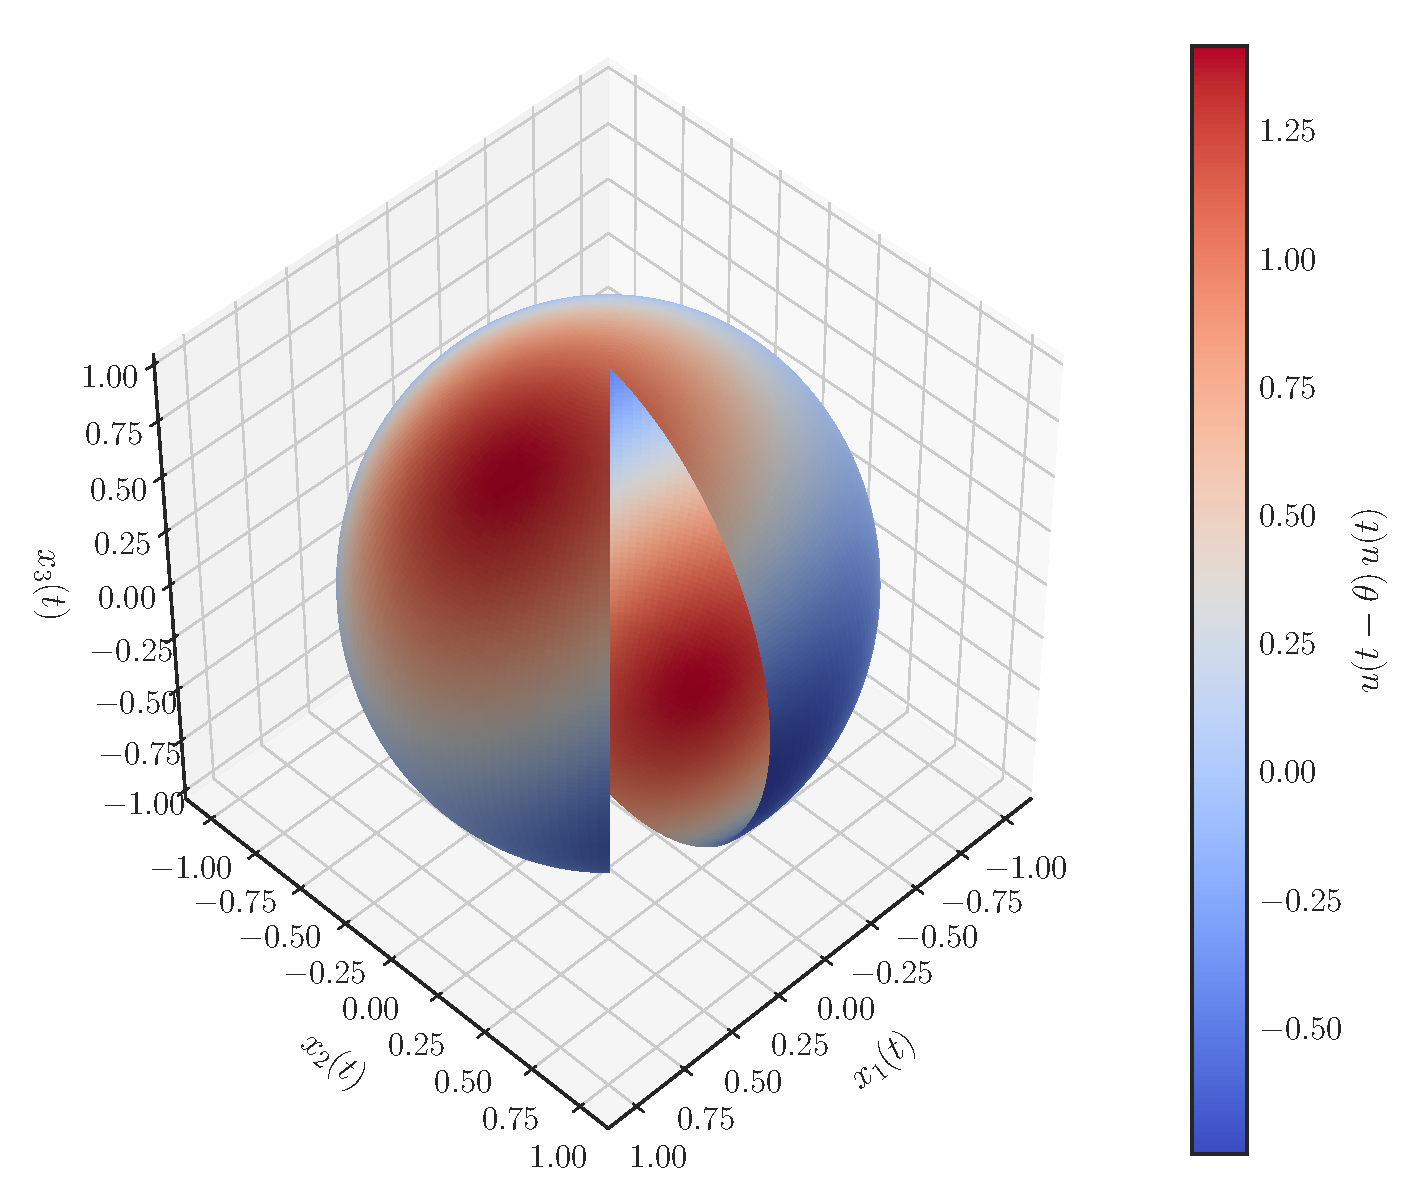
\includegraphics[width=0.5\linewidth]{delay-autocorrelation}
  \caption{ \label{fig:delay-autocorrelation} 
    Visualizing the autocorrelation function $y(t) = u(t - \theta)\, u(t)$ with $q=3$.
    Each point along the surface of the unit-sphere is $\V{x}(t)$, and is coloured according to its corresponding value of $y(t)$ obtained from equation~\ref{eq:basis-interpretation}.
    A slice of the shell is cut away for visualization.
  } 
\end{figure}

\subsection{Scalability considerations}
\label{sec:delay-scalability}

\begin{figure}
\centering
  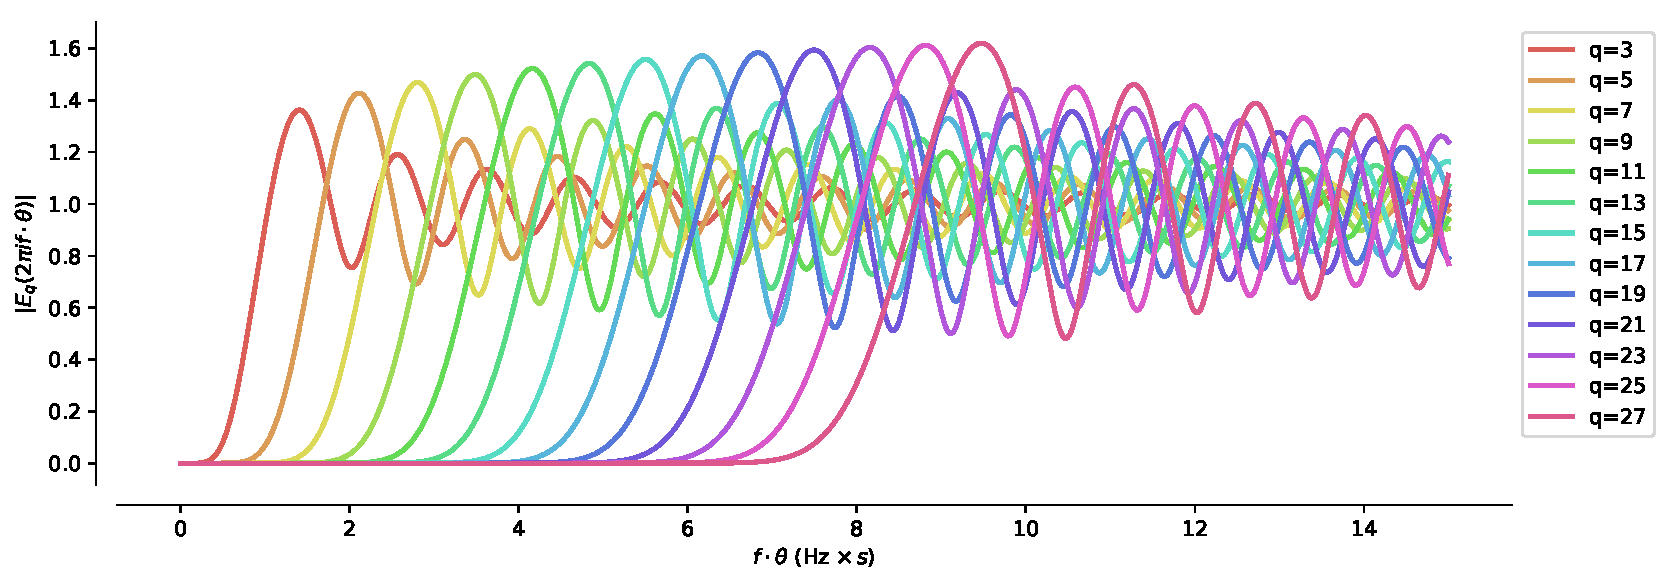
\includegraphics[width=1.0\linewidth]{pade-delay-error}
  \caption{ \label{fig:pade-delay-error} 
    Visualizing the error in the Delay Network, $|E_q(2 \pi i f \cdot \theta)|$ (see equation~\ref{eq:pade-delay-error}), while varying the dimensionless quantity $f \cdot \theta$ (input frequency multiplied by delay length), and the order of approximation, $q$.
  } 
\end{figure}

In this section we address several fundamental questions regarding the scalability, or memory ``capacity'', of the Delay Network~(DN) with respect to $q$, $\theta$, and the complex frequency of the input signal, $s = 2 \pi i f$, for some real frequency, $f$.
For the time being, we disregard the error arising from neural representation by assuming we can make $n$ sufficiently large (see section~\ref{sec:scalability}).
This means we match the model description precisely, even when considering more elaborate models of the synapse (see chapter~\ref{sec:synaptic-extensions}).
The only source of error remaining is our use of Pad\'e approximants to render equation~\ref{eq:tf-delay} finite-dimensional.
This error term may be expressed in the Laplace domain as follows:
\begin{equation} \label{eq:pade-delay-error}
E_q(\theta s) = [q-1/q]e^{-\theta s} - e^{-\theta s} \text{,}
\end{equation}
where $[q-1/q]e^{-\theta s}$ is defined by equation~\ref{eq:pade} (see Figure~\ref{fig:pade-delay-error}).\footnote{%
For example, $|E_{21}(2 \pi i \cdot 5)| \approx 0.003$ implies that a $21$-dimensional DN delays a $1$\,Hz signal for $5$\,s with $0.3\%$ error.}
By linearity of the Laplace transform, it suffices to consider the error at individual frequencies $s$ in order to fully characterize the error of the entire system for any given input.
More precisely, by the convolution theorem, we can interpret equation~\ref{eq:pade-delay-error} as a linear filter in the $s$-plane, to reveal how each input frequency is amplified, attentuated, or phase-shifted, to contribute to the spectrum of the overall error.\footnote{%
Only frequencies that are present within the input can become present in the error.}

Dimensional analysis quickly reveals an important property of this error: the dimensionless quantity, $\theta s$ (i.e., the product of time and frequency), fully determines the error (for fixed $q$).
In other words, the ``difficulty'' of computing a delay is a function of the length of the delay multiplied by the frequency of the input signal being delayed.
For instance, delaying a $10$\,Hz signal for $0.1$\,s has the same approximation error as delaying a $0.1$\,Hz signal for $10$\,s.
This is seen by simply rescaling the time-axis by a factor of $100$.
This is also consistent with the results from Figure~\ref{fig:delay-full}.

This is deeply connected to the observation that in equation~\ref{eq:ss-delay}, the delay length $\theta$ scales inversely with the gain on $A$ and $B$.
The identification of this control factor can be derived from a more general property of the Laplace transform, $F \left( \theta s \right) = \theta^{-1} \mathcal{L} \left\{ f \left( t / \theta \right) \right\} (s)$ for all $\theta > 0$, meaning that the time-scale of any linear filter is rescaled by a gain on the integration.
We can exploit this fact more generally to modulate the time-scale of any linear filter on-the-fly (in this case affecting the length of delay; results not shown).

Next, as shown in Figure~\ref{fig:pade-delay-error}, the radius of convergence for the Pad\'e approximants increases linearly with $q$.\footnote{%
We have increased $q$ as large as $80$ before running into numerical issues related to catastrophic cancellation and discretizing the system via zero-order hold.
We are confident that these issues can be resolved by more careful use of numerical methods, due to the isomorphism between our delay polynomials and the shifted Legendre polynomials.}
Thus, scaling $q$ by some factor means that either the frequency of the input signal or the length of the delay can be scaled by the same factor, while achieving the same error.
When $\theta s$ is outside the radius of convergence, the absolute error is bounded between $0$ and $2$.
This fact simply comes from the observations that $e^{-\theta s}$ is a unit-length complex number, and $[q-1/q]e^{-\theta s}$ is complex with magnitude less than $1$.
Thus, by the triangle inequality, the magnitude of their difference is bounded above by $2$.
In the limit as $\theta s \rightarrow \infty$, the magnitude of the error converges to $1$ as $[q-1/q]e^{-\theta s} \rightarrow 0$.

We may interpret these results in the context of equation~\ref{eq:pade-delay-error} as a linear filter.
When $\theta s$ is small (within the radius of convergence, which scales linearly with $q$), an input frequency at $s$ radians is delayed almost perfectly for $\theta$ seconds.
Outside the radius of convergence, the error contains frequencies that are phase-shifted and multiplied (with magnitude bounded above by $2$) versions of the input frequencies in that range.
As $\theta s$ increase further, the error contains input frequencies that are simply phase-shifted, without any change in magnitude.

Lastly, as revealed by equation~\ref{eq:basis-functions}, and as shown in Figure~\ref{fig:basis-functions}, the basis functions are also dimensionless, in the sense that they are defined over the range $r \in [0, 1]$ which maps onto the time-interval $(t - \theta') \in [t - \theta, t]$, where $\theta' = r \theta$, for any $\theta > 0$.
This has numerous consequences that are intertwined: (1) the relationship between the input signal and its state-vector is scale-invariant; scaling the input length by some factor, and the delay length by the same factor, results in the exact same state-vector corresponding to a rescaled input history, (2) we can perform computations on the representation of the DN, independently of scale; see section~\ref{sec:periodicity} for an example, and (3) we can reinterpret the same state-vector with respect to any time-scale without changing the state-vector.

Taking neural constraints into consideration, we do need to separate out $\theta s$ into its dimensional quantities.
As shown in section~\ref{sec:poisson-spiking}, the frequency of the state-vector being represented can matter.
This concern is resolved by the use of Poisson spiking, integrate-and-fire neurons, or any other solution to state discrepancy (section~\ref{sec:spike-coding}).
On the other hand, longer values of $\theta$ are more susceptible to the integration of spiking noise, in the form of ``drift''.
Lastly, when using a balanced realization, larger values of $q$ require denser interconnectivity ($q \times q$ transform matrices) between all $q$ dimensions, leading to $\bigoh{q^2}$ increase in time and memory requirements.
Such considerations are addressed in section~\ref{sec:deep-delay-networks} by stacking multiple DNs together to form a Deep Delay Network~(DDN).

To summarize, the properties of scaling $\theta$ are physically coupled to considerations of which input frequencies need to be delayed, and to what degree of precision.
The accuracy is a function of $\theta s$.
And, for a fixed level of precision, $\theta s$ scales linearly with $q$.
In all cases, the representation employed by the DN (i.e., the linear relationship between the input history and the state-vector) is scale-invariant in $\theta$.

\section{Applications}
\label{sec:delay-applications}

We have developed rigorous theory to understand the Delay Network~(DN) in terms of its linear dynamics, and its nonlinear encoding of time, and used the NEF to present a spiking example in Figure~\ref{fig:delay-example}.
Now, we turn to several concrete applications that are of relevance to those studying reservoir computing, FORCE learning, deep RNNs and stacked LSTMs, as well as the computational neuroscience and cognitive modelling communities at large.

\subsection{Reservoir Computing}
\label{sec:delay-rc}

Here we show that the NEF provides a principled way to optimize a particular RNN architecture, by mapping the desired dynamical state onto a latent representation within a factorable connection weight matrix (also see sections~\ref{sec:engineered-approaches} and~\ref{sec:relationships}).
This enables us to train networks that outperform Reservoir Computing~(RC) methods---using either spiking~\citep[LSM;][]{maass2002real} or rate-based~\citep[ESN;][]{jaeger2001echo} neurons---in memory capacity and nonlinear computation, while reducing the simulation time and space requirements by a factor of $\bigoh{n}$.
%These same results carry over to FORCE, state-of-the-art ``full-FORCE'' methods, and even stacked LSTMs, in the following section.
Our approach can learn both online and offline, readily incorporates detailed synapse models, supports various spiking and rate-based neuron models, and may be compiled onto analog and digital neuromorphic hardware.

\subsubsection{Linear benchmark}

Training a network to implement a delay is a natural way to measure the dynamical system's memory capacity---its ability to maintain a history of its input signal---which is needed to compute any function over past inputs.
Indeed, this task was considered by ESNs in one of the earliest demonstrations of the RC paradigm~\citep{jaeger2002short}.  In its purest analog form, a delay line is attempting to encode an infinite amount of information, which is why it is a challenging and useful benchmark to consider.
Theoretical and experimental results in the past have pointed to the limited capability of random feedback to maintain memory~\citep{joshi2005movement, mayor2005signal, dambre2012information, wallace2013randomly, inubushi2017reservoir, schuecker2018optimal}, in particular finding that linear feedback \emph{maximizes} memory capacity~\citep{mitra2001nonlinear}---as derived in section~\ref{sec:nef-delay}, and considering the linearity of a delay line---while being at odds with the nonlinearities that are required to support useful computations across the memory.\footnote{%
We thank Kwabena Boahen for pointing out this connection and a few of these references.
}
This is consistent with our findings below.
Moreover, the DN poses a natural way out of this predicament, by using nonlinearities to approximate the required linear feedback, without sacrificing the ability to nonlinearly transform the window (section~\ref{sec:delay-nonlinear} and below).

For our benchmark task, weights were trained and validated using randomly sampled $25$\,Hz band-limited white noise inputs.
In addition, full-spectrum white noise was added to the network during both training and testing.
Accuracy was measured by normalizing the root-mean squared error against the root-mean squared target~\citep[NRMSE;][]{lukovsevicius2012reservoir}.
As well, $95\%$ confidence intervals were bootstrapped and plotted using Seaborn~\citep{michael_waskom_2015_19108}.
We ported a Python implementation of the ESN from \cite{lukovsevivcius2009reservoir} to Nengo, and implemented it analogously to the DN.
Nengo allows us to consider populations of either spiking LIF neurons or non-spiking neurons with various rate curves, without any additional changes to the model specification.
In particular, LSMs were implemented by replacing the $\tanh$ units with LIF spiking neurons, making them comparable to our NEF networks but with full-rank weight matrices.
The hyperparameters of each method were optimized using $200$ iterations of HyperOpt~\citep{bergstra2013making} with $3$ trials per iteration, to maximize the validation error for $200$\,ms delays (see Table~\ref{tab:hyperopt}).
Hyperparameters include an overall gain on the recurrent feedback matrix (gain), a normalization factor for the input (radius), time-constants on both the readout and recurrent filters ($\tau_\text{readout}$, $\tau_\text{recurrent}$), L2-regularization parameters for applicable least-squares problems ($\sigma^2_\text{readout}$, $\sigma^2_\text{recurrent}$), and the dimensionality of the delay network ($q$).\footnote{%
HyperOpt was used to the benefit of LSMs and ESNs. All hyperparameters (apart from $q$) had minimal effect on the DN's performance compared to the usual defaults in Nengo.}
%All data and figures may be reproduced by following the instructions at the following URL: \path{https://github.com/arvoelke/rc2017}.

\begin{figure}
\centering
  \begin{tikzpicture}[auto, >=latex']
    \node [input, label=left:{$u[t]$}] (u) {};
    \node [block, right of=u, node distance=2cm] (h) {$h[t]$};
    \node [ensemble, right of=h, node distance=2cm] (x) {$\V{x}[t]$};
    \node [output, label=right:{$y[t]$}, right of=x, node distance=1.5cm] (y) {};
    \draw [->] (u) -- node {$\bar{B}^H$} (h);
    \draw [->] (h) -- (x);
    %\draw [->] (x.north) -- (y);
    \draw [->] (x) -- (y);
    %\draw [->] (x.south) -- (y);
    \path[->] (x.south) edge [loop below, min distance=5em, out=-60, in=-120] node {$\bar{A}^H$} (h.south);
  \end{tikzpicture}
  \caption{ \label{fig:delay-architecture}
    Delay Network~(DN) model for a digital architecture.
    The synapse $h[t]$ is driven by $\bar{A}^H \V{x}[t] + \bar{B}^H u[t]$ to yield the state $\V{x}[t]$.
    This state is nonlinearly encoded by a heterogeneous population of neurons and subsequently decoded to estimate the desired $y[t]$.
  } 
\end{figure}

In all cases, we construct a reservoir of $\numprint{1500}$ neurons, and then train separate linear readouts to approximate various delays ranging from $100$--$200$\,ms ($\dt{} = 1$\,ms).
For the NEF case, the prescribed dynamical system is a $\theta = 200$\,ms delay, implemented by mapping equation~\ref{eq:ss-delay} onto a discretized lowpass (see equation~\ref{eq:discrete-p3}).
In section~\ref{sec:delay-lstm} we show that the delay length can be trained from raw data.
Importantly, the same networks are used to compute all of the different delays reported.
We thus conceptualize the DN as an optimized ``low-dimensional reservoir''.
%The input to each network is randomly sampled $25$\,Hz band-limited white noise.
Compiling all of the equations of this network, for clarity (see Figure~\ref{fig:delay-architecture}):
\begin{equation} \label{eq:delay-compiled}
\begin{aligned}
v_i &= \frac{(q+i)(q-i)}{i+1} \theta^{-1} \text{,} \quad i = 0 \ldots q-1 \\
A &= \begin{pmatrix} -v_0 & -v_0 & \cdots & -v_0 \\ v_1 & 0 & \cdots & 0 \\ 0 & \ddots & \ddots & \vdots \\ 0 & 0 & v_{q-1} & 0\end{pmatrix} \in \mathbb{R}^{q \times q} \\
B &= \transpose{\begin{pmatrix} v_0 & 0 & \cdots & 0\end{pmatrix}} \in \mathbb{R}^{q} \\
\bar{A} &= \sum_{i=0}^\infty c_i A^i = \sum_{i=0}^\infty \frac{\left(A\dt{}\right)^i}{i!} = e^{A\dt{}}  \\
\bar{B} &= \left( \sum_{i=1}^\infty c_i A^{i-1} \right) B = A^{-1} \left(\bar{A} - I\right) B  \\
a &= e^{-\frac{\dt{}}{\tau}} \\
\bar{A}^H &= \frac{1}{1 - a} \left(\bar{A} - aI\right) \\
\bar{B}^H &= \frac{1}{1-a}\bar{B} \text{.}
\end{aligned}
\end{equation}
We remind the reader that $A$ and $B$ may be transformed by any of the state-space realizations from section~\ref{sec:software} before proceeding with the remaining numerical machinery.
The final matrices $(\bar{A}^H\text{,}\, \bar{B}^H)$ determine the transformations to be implemented using Principles~1 and~2 of the NEF, which in turn will nonlinearly encode $\V{x}[t]$ by our extensions to Principle~3.

\begin{figure}
  \centering
  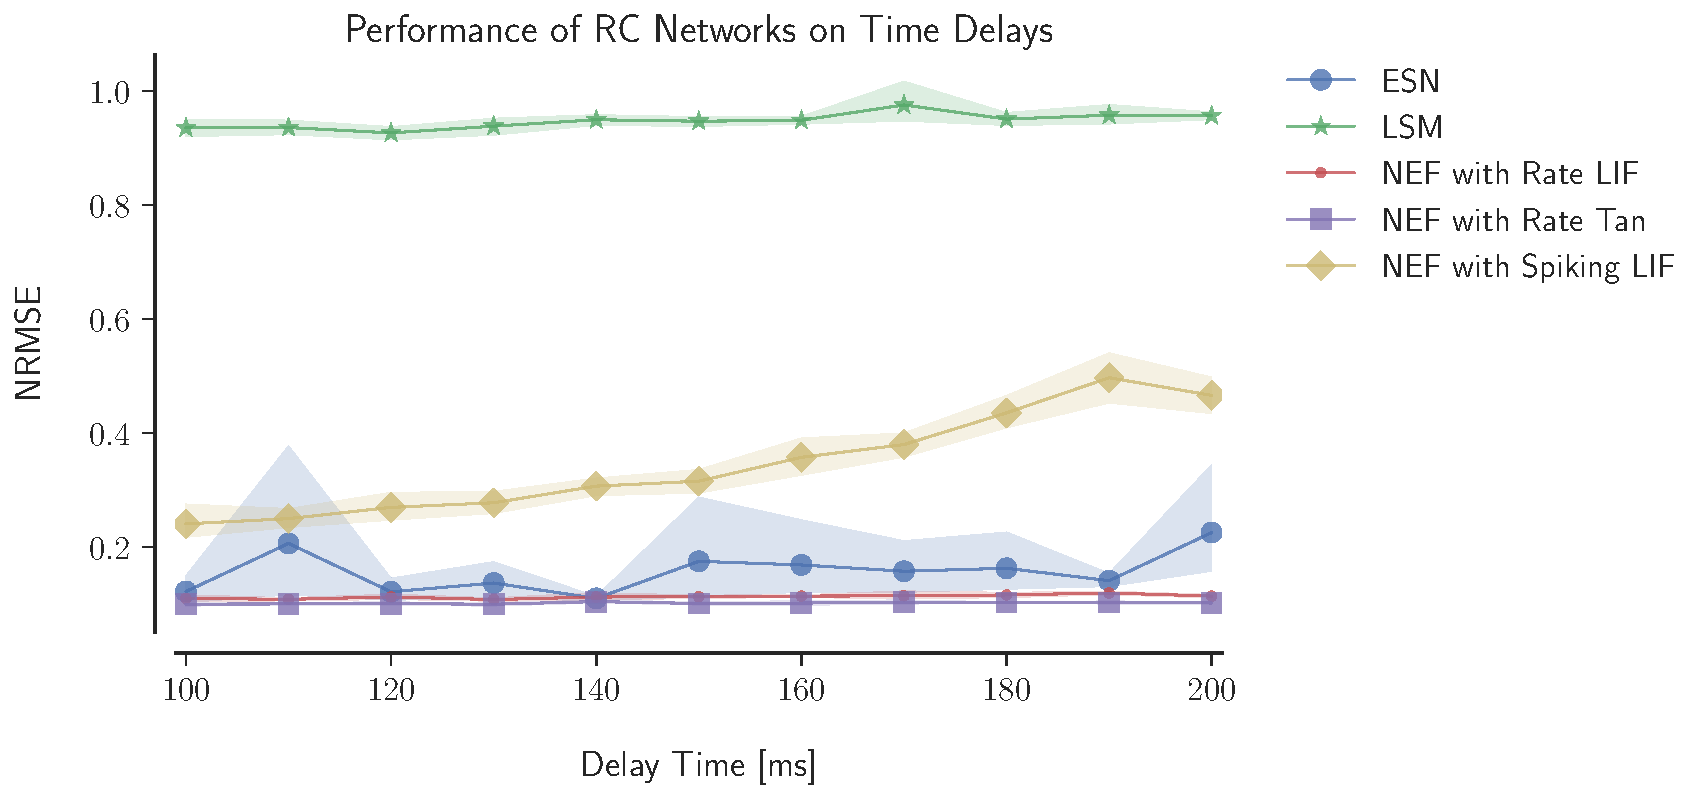
\includegraphics[width=0.8\textwidth]{rc-accuracy}
  \caption{ \label{fig:rc-accuracy}
  Performance from training various linear readouts to compute delays of $25$\,Hz band-limited white noise (bootstrapped across 10 trials).
  Each line corresponds to a single reservoir of $\numprint{1500}$ neurons, either randomly connected (in the case of ESNs and LSMs), or specifically engineered (in the case of the NEF).
  }

  \vspace{1em}

  \centering
  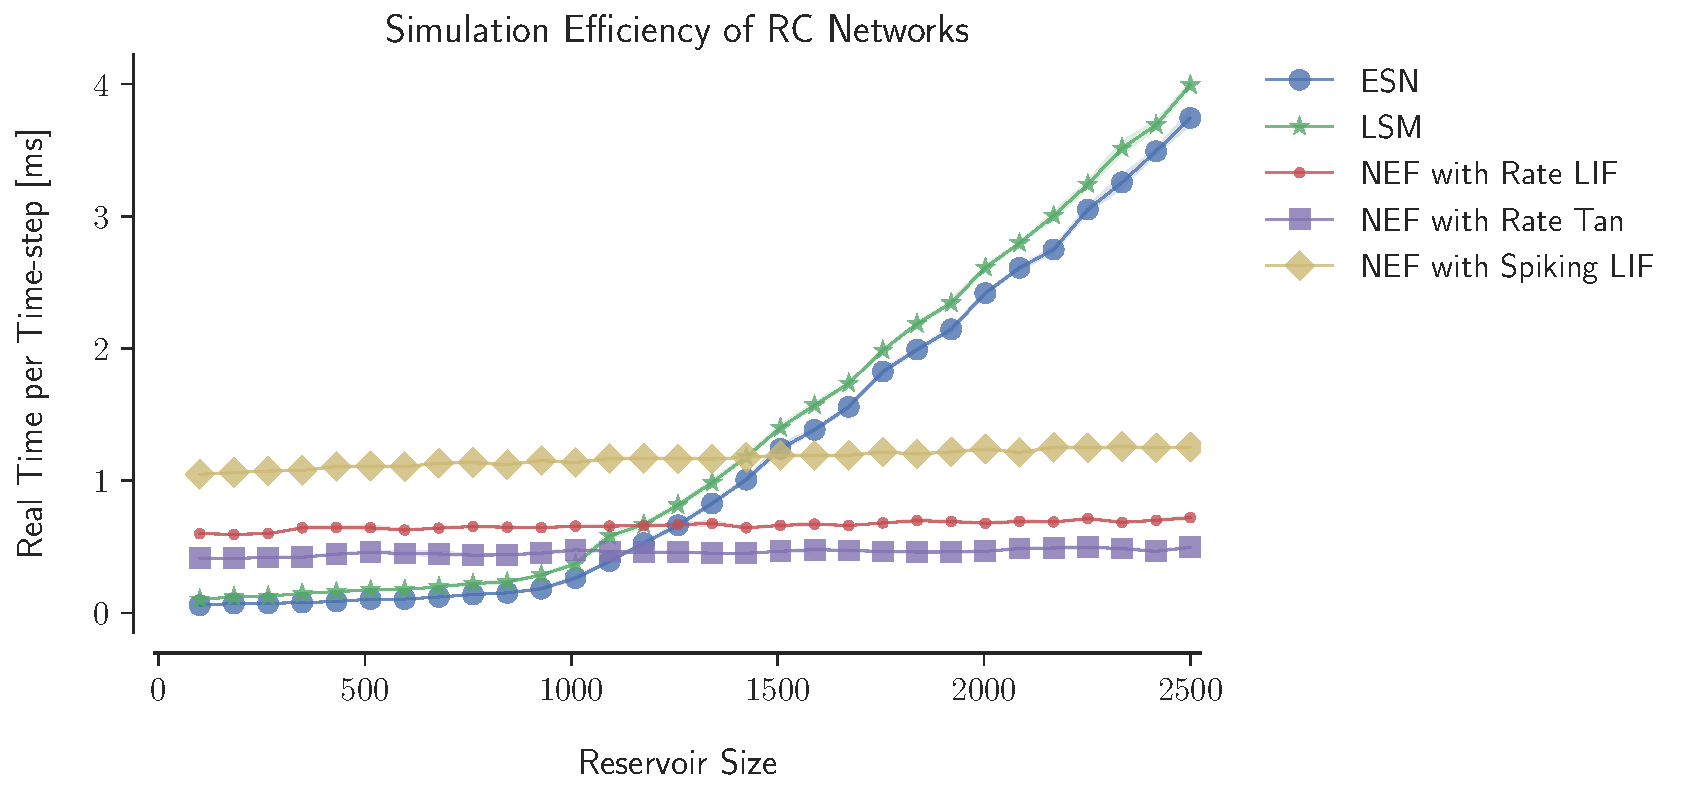
\includegraphics[width=0.8\textwidth]{rc-speed}
  \caption{ \label{fig:rc-speed}
  Cost of simulating each RC network as the reservoir size is increased (bootstrapped across 10 trials).
  Conventional RC approaches require $\bigoh{ n^2 }$ space and time, while the NEF improves this to $\bigoh{ n }$ for constant dimensionality.
  }
\end{figure}

As shown in Figure~\ref{fig:rc-accuracy}, the NEF's performance is slightly better than ESNs for both LIF rate neurons and $\tanh$ rate neurons, and significantly better than LSMs for spiking LIF neurons.
This demonstrates that, in terms of memory capacity, the DN as a low-dimensional reservoir not only outperforms RC in the rate-based case, but even performs comparably to ESNs when using spikes.
The task is shown to be completely outside the grasp of LSMs (exceeding $90$\% error), due to the difficulty of the computation and the unreliability of randomized spiking feedback; HyperOpt minimizes both the gain and regularization hyperparameters of the LSM to keep its output close to zero, as this minimizes validation error.\footnote{%
As additional validation, lower input frequencies or shorter delay lengths were possible with the LSM.}
The success of the DN should not be surprising given that we have mapped the ideal delay's dynamics onto the reservoir.
Nevertheless, as we will show below, the readouts are capable of computing nonlinear functions across the delay interval, from the same reservoir.
%This demonstrates that our derived state-vector (see Figure~\ref{fig:pca}) is robust to changes in the target function.
Informally, assigning some particular dynamics to the reservoir does not disable the network from computing other similar functions (thereby permitting nonlinear combinations of such functions to be trained from data).

These networks were also simulated while varying the number of neurons from $100$ to $\numprint{2500}$, in order to measure the real-time cost of simulation (see~Figure~\ref{fig:rc-speed}).
We again note that traditional RC suffers from scaling issues since the recurrent weight matrices have $\bigoh{ n^2 }$ coefficients.
Consequently, the NEF is more resource efficient than these RC methods by a factor of $\bigoh{ n }$.
RC networks often include a sparsity constraint of $20\%$ connectivity, which is still $\bigoh{n^2}$, in order to improve performance~\citep{lukovsevivcius2012practical, lukovsevicius2012reservoir}.
We also considered ESNs with constant sparsity that balance resource constraints with NEF networks, but found that they did not perform comparably (not shown).
Furthermore, we found that the ESN breaks down for numbers of neurons as few as $q$ neurons, while in fact $q$ linear rate neurons (with linearly independent encoders) will suffice to perfectly implement equation~\ref{eq:ss-delay}, as $q$ linear state-variables are in exact correspondence with the ideal linear system (after the appropriate discretization of equation~\ref{eq:discrete-p3}) (see section~\ref{sec:force-comparison}).

\begin{table}\centering
  %\ra{1.2}
  \noindent\begin{tabularx}{\textwidth}{YYYYYY}
    \toprule
     & ESN & LSM & NEF with Rate LIF & NEF with Rate Tan & NEF with Spiking LIF \\
    \midrule
Gain & \num[round-precision=3,round-mode=figures,scientific-notation=true]{1.3251896701} & \num[round-precision=3,round-mode=figures,scientific-notation=true]{0.00315170551016} & - & - & - \\

Radius & \num[round-precision=3,round-mode=figures,scientific-notation=true]{24.3145093319} & \num[round-precision=3,round-mode=figures,scientific-notation=true]{1.36259213791} & \num[round-precision=3,round-mode=figures,scientific-notation=true]{4.63655157006} & \num[round-precision=3,round-mode=figures,scientific-notation=true]{12.8794579757} & \num[round-precision=3,round-mode=figures,scientific-notation=true]{0.577484080063} \\

$\tau_\mathrm{readout}$ & \num[round-precision=3,round-mode=figures,scientific-notation=true]{0.00686793487811} & \num[round-precision=3,round-mode=figures,scientific-notation=true]{0.0604400629751} & \num[round-precision=3,round-mode=figures,scientific-notation=true]{0.0606008691858} & \num[round-precision=3,round-mode=figures,scientific-notation=true]{0.0873173665926} & \num[round-precision=3,round-mode=figures,scientific-notation=true]{0.0218081523547} \\

$\tau_\mathrm{recurrent}$ & \num[round-precision=3,round-mode=figures,scientific-notation=true]{0.0021441109352} & \num[round-precision=3,round-mode=figures,scientific-notation=true]{0.069089989522} & \num[round-precision=3,round-mode=figures,scientific-notation=true]{0.0626041764586} & \num[round-precision=3,round-mode=figures,scientific-notation=true]{0.0937145408042} & \num[round-precision=3,round-mode=figures,scientific-notation=true]{0.0740410932649} \\

$\sigma^2_\mathrm{readout}$ & \num[round-precision=3,round-mode=figures,scientific-notation=true]{2.95578336256e-06} & \num[round-precision=3,round-mode=figures,scientific-notation=true]{0.0329425610169} & \num[round-precision=3,round-mode=figures,scientific-notation=true]{0.00206289719197} & \num[round-precision=3,round-mode=figures,scientific-notation=true]{0.00479755699712} & \num[round-precision=3,round-mode=figures,scientific-notation=true]{0.0450158827701} \\

$\sigma^2_\mathrm{recurrent}$ & - & - & \num[round-precision=3,round-mode=figures,scientific-notation=true]{0.000200121787175} & \num[round-precision=3,round-mode=figures,scientific-notation=true]{0.000397747221121} & \num[round-precision=3,round-mode=figures,scientific-notation=true]{0.0375517001869} \\

$q$ & - & - & 20 & 26 & 23 \\

    \bottomrule
  \end{tabularx}
  
  \caption{ \label{tab:hyperopt}
    HyperOpt parameters for the linear benchmark in section~\ref{sec:delay-rc}.
  }
\end{table}

Another key finding is that, as shown in Table~\ref{tab:hyperopt}, 
HyperOpt discovers that a radius of $\approx 24.3$ performs the best with the ESN.
This has the effect of scaling the domain of the tanh curve from $[-1, 1]$ to $\approx [-0.04, 0.04]$, which importantly is well-approximated by a straight line, that is, $\tanh x \approx x$ across this domain.
Thus, HyperOpt is indirectly leveraging the fact that the ESN's memory capacity is maximized when its neurons \emph{are linear}, consistent with \citet{dambre2012information}.
Crucially, this limits the ability of the ESN to perform nonlinear computations across the delay interval, as we now show.

\subsubsection{Nonlinear benchmark}

To demonstrate our ability to compute nonlinear window functions, we consider the function from section~\ref{sec:delay-nonlinear}, $y(t) = u(t - \theta)\, u(t)$, visualized in the context of a DN's state-vector in Figure~\ref{fig:delay-autocorrelation}.
When integrated over time, this is the autocorrelation of $u$ with lag $\theta$, which has numerous applications in signal processing (e.g.,~detecting repeating events).
We fix $\theta = 0.1$\,s across all experiments.
To compute this function accurately, we sample a proportion of the encoders from the diagonal combinations of $\mathcal{P}_{i, d}(0)$ and $\mathcal{P}_{i, d}(1)$~\citep{jgosmann2015}.
However, the particular choice of function is not of importance, as the training can be data-driven, or analyzed using theory from sections~\ref{sec:temporal-representation} and~\ref{sec:delay-nonlinear}.

Each input $u(t)$ is sampled white noise, band-limited with a cutoff frequency of $30$\,Hz.
To optimize for the decoders, we map $q$-dimensional evaluation points onto desired target outputs using equation~\ref{eq:basis-interpretation}, and apply Nengo's regularized least-squares solver, which bypasses the need to explicitly simulate the network on any input signals.

To implement this system as a spiking (or non-spiking) recurrent neural network, we use the same set of transformations from equation~\ref{eq:delay-compiled}. % Principle~3 of the NEF to map equation~\ref{eq:delay-system} onto the dynamics of the synapse.
%For example, repeating the standard form of Principle~3 for a continuous-time lowpass synapse with time-constant $\tau$ (although we are free to use the extensions of chapter~\ref{chapt:nef-extensions}):
%\begin{equation} \label{eq:delay-system-p3}
%A^H = \tau A + I \text{,} \quad B^H = \tau B \text{,} \quad H(s) = \left(\tau s + 1\right)^{-1} \text{.}
%\end{equation}
The model architecture of this delay network is, again, depicted in Figure~\ref{fig:delay-architecture}, whose representation and transformations are realized using the NEF.
For this experiment, we considered the use of both sigmoidal (non-spiking) neurons, and spiking LIF neurons.

We again used HyperOpt~\citep{bergstra2015hyperopt} to explore the space of model hyperparameters (e.g.,~$q$, $\tau$, input gain, recurrent gain, L2-regularization) across $100$ iterations containing $10$ trials each.
Each network consisted of $\numprint{1000}$ neurons, simulated with a time-step of $\dt{} = 1$\,ms.
Each trial used a training signal of length $\numprint{10200}$, a testing signal of length $\numprint{2200}$, and the first $200$ outputs were discarded.
We then cross-validated the best set of hyperparameters (in terms of mean NRMSE across all test signals) using another $25$ trials.

We obtain a mean NRMSE of $5.9$\% for the sigmoid DN, $51.8$\% for the spiking DN, and $84.3$\% for the $\tanh$ ESN.
Reducing the input frequency from $30$\,Hz to $15$\,Hz improves the ESN's accuracy to be on par with the non-spiking DN, and thus we attribute this difference to the inherent difficulty of autocorrelating a high-frequency signal (relative to $\theta$) using random feedback weights, as opposed to using optimally derived weights as in the DN.
In addition, trials took on average $5.10$\,s for the sigmoid DN, $6.44$\,s for the spiking DN, and $17.7$\,s for the ESN.
This difference is a consequence of not simulating the DN for training, and from using factorized weight matrices (i.e.,~encoders and decoders) to simulate the DN.
These results are consistent with that of the linear benchmark, except for the additional observation that here the spiking DN outperforms the rate ESN.
This is because, as explained previously, the ESN's memory capacity requires linear tuning, which is at odds with the nonlinearities required by functions such as autocorrelation.
LSMs were again unable to perform.


\subsection{FORCE learning}
\label{sec:force-comparison}

We also compared our NEF solution to both FORCE~\citep{sussillo2009generating} and full-FORCE~\citep{depasquale2018full} networks (also see sections~\ref{sec:engineered-approaches} and~\ref{sec:relationships}).
FORCE networks take the same essential ingredient of RC networks, namely the inclusion of high-dimensional random feedback, except they make an important addition to the model: the target output is learned---online via RLS---to be simultaneously re-encoded back into the network (see Figure~\ref{fig:architectures}).
Full-FORCE takes this a step further, by using the postsynaptic currents from the previous FORCE network as a training signal for a separate ``full-FORCE'' network. 
In the first step, the FORCE network does not do any online learning, but instead receives the exact ideal teaching signal.
The second step then allows for additional degrees of freedom to be optimized, to find the \emph{full weights} that reconstruct the ideal PSCs from the first network -- again, online using RLS.
This is similar in many ways to \citet{tripp2006neural}, but maintains the same idea as in FORCE, in particular the re-encoding of the target state.
The main difference from FORCE is that instead of learning a low-rank (one-dimensional) decode-encode of the target, full-FORCE learns a full-rank approximation to an encoding of that same target.

For this experiment, we first ported the same implementation described in \citet{depasquale2018full} to Nengo, and verified that it is works as intended (using the same models and parameters) by teaching the network to produce decaying oscillations in response to unit impulses.
We compared this to the standard FORCE approach---which we refer to as ``classic-FORCE''---and verified that it performed slightly worse than the full-FORCE network, but still better than an equivalent reservoir computer.
Since Nengo allows for the substitution of various spiking and non-spiking neuron models, we further validated both implementations with spiking neurons as well, and obtained reasonable levels of accuracy, similar to \citet{depasquale2016using, thalmeier2016learning, nicola2016supervised}.

However, we found that simply modifying the target signal to be a delayed version of a low-frequency signal, posed an incredible challenge for these networks.
Thus, the learning rate was lowered from $1$ to $\numprint{e-3}$, and the time-step set to $\dt{} = 5$\,ms, which we found to help regularize the solution.
We thus also considered a baseline approach:
we took the original FORCE network, but removed the feedback loop that re-encodes the learned output.
This makes it equivalent to an ESN with a slightly different method of distributing the weights, while learning the decoders online.
We refer to this last method as ``no-FORCE''.

Finally, we compared all three of these to an idealized NEF implementation of the DN~(equation~\ref{eq:ss-delay}), consisting of just $n = 6$ linear units, coupled to one another by the discretized mapping of equation~\ref{eq:discrete-p3}, as summarized by equation~\ref{eq:delay-compiled} ($q = 6$).
In this scenario, the only error that remains is that of equation~\ref{eq:pade-delay-error} arising from the use of Pad\'e approximants to render the delay line finite-dimensional.
In all cases, the training and test signals were randomly sampled $1$\,Hz band-limited white noise signals.
We compared all four networks by sweeping $\theta$ across $0.01$--$1$\,s, with $10$ trials at each condition (boostrapped 95\% confidence intervals).
Figure...\TODO{Figure}

\subsection{Long short-term memory}
\label{sec:delay-lstm}

\subsection{Time cell data}
\label{sec:time-cells}

This section has been reproduced from \citet{voelker2018}.

We now describe a connection between the delay network from this chapter and recent neural evidence regarding time cells.
Time cells were initially discovered in the hippocampus and proposed as temporal analogs of the more familiar place cells~\citep{eichenbaum2014}.
Similar patterns of neural activity have since been found throughout striatum~\citep{mello2015scalable} and cortex~\citep{luczak2015packet}, and have been extensively studied in the rodent mPFC~\citep{kim2013neural, tiganj2016sequential}.

Interestingly, we find that our delay network produces qualitatively similar neural responses to those observed in time cells.
This is shown in Figure~\ref{fig:time-cells}, by comparing neural recordings from mPFC~\citep[][Figure~4~C,D]{tiganj2016sequential} to the spiking activity from a network implementing a delay of the same length used in the original experiments.
Specifically, in this network, a random population of $300$ spiking LIF neurons maps a $4.784$\,s\footnote{%
This value comes from \citet{tiganj2016sequential}.}
delay onto an alpha synapse ($\tau = 0.1$\,s) using our extension.
The order of the approximation is $q = 6$ (see equation~\ref{eq:ss-delay}), and the input signal is a rectangular pulse beginning at $t = -1$\,s and ending at $t = 0$\,s (height $= 1.5$).
The simulation is started at $t = -1$\,s and stopped at $t = 5$\,s.

\begin{figure}
  \centering
  \includegraphics[width=\textwidth]{{NECO-04-17-2838-Figure.10-Top}.pdf}
  \includegraphics[width=0.96\textwidth, trim=0 0 -0.7in -0.4in]{{NECO-04-17-2838-Figure.10-Bottom}.pdf}
  \caption{ \label{fig:time-cells}
    Comparison of time cells to a NEF delay network.
    (Top)~Spiking activity from the rodent mPFC~\citep[reproduced from][Figure~4~C,D]{tiganj2016sequential}.
    Neural recordings were taken during a maze task involving a delay period of $4.784$\,s.
    (Bottom)~Delay network implemented using the NEF (see text for details).
    %A random population of $300$ spiking LIF neurons map a $4.784$\,s delay onto an alpha synapse ($\tau = 0.1$\,s) using equation~\ref{eq:general-linear-approx}.
    %The order of the approximation is $q = 6$ (see equation~\ref{eq:ss-delay}), and the input signal is a rectangular pulse beginning at $t = -1$\,s and ending at $t = 0$\,s.
    $73$ time cells are selected by uniformly sampling encoders from the surface of the hypersphere.
    (A)~Cosine similarity between the activity vectors for every pair of time-points.
    The diagonal is normalized to the warmest colour.
    The similarity spreads out over time.
    (B)~Neural activity sorted by the time to peak activation.
    Each row is normalized between $0$ (cold) and $1$ (warm).
    We overlay the curve from Figure~\ref{fig:pca}(Bottom) ($q = 6$) to model the peak-response times.
  }
\end{figure}

We also note a qualitative fit between the length-curve for $q=6$ in Figure~\ref{fig:pca} and the peak response-times in Figure~\ref{fig:time-cells}.
Specifically, Figure~\ref{fig:pca}(Bottom) models the non-uniform distribution of the peak response-time of the cells as the length of the trajectory of $\V{x}(t)$ through time.
Implicit to this model are the simplifying assumptions that encoders are uniformly distributed, and that the L2-norm of the state-vector remains constant throughout the delay period.
Nevertheless, this model produces a qualitatively similar curve when $q = 6$ to both peak response-times from Figure~\ref{fig:time-cells}(Right) (see overlay).

More quantitatively, we performed the same analysis on our simulated neural activity as \citet{tiganj2016sequential} performed on the biological data to capture the relationship between the peak and width of each time cell.
Specifically, we fit the spiking activity of each neuron with a Gaussian to model the peak time~($\mu_t$) and the standard deviation~($\sigma_t$) of each cell's ``time field''.\footnote{%
We set $a_1 = P = S = 0$ in equation~1 from \citet{tiganj2016sequential}, since we have no external variables to control.
}
This fit was repeated for each of the $250$ simulated spiking LIF neurons that remained after selecting only those that had at least $90\%$ of their spikes occur within the delay interval.
The correlation between $\mu_t$ and $\sigma_t$ had a Pearson's coefficient of $R = 0.68$ ($\rho < \numprint{e-34}$), compared to $R = 0.52$ ($\rho < \numprint{e-5}$) for the biological time cells.
An ordinary linear regression model linking $\mu_t$ (independent variable) with $\sigma_t$ (dependent variable) resulted in an intercept of $0.27 \pm 0.06$ (standard error) and a slope of $0.40 \pm 0.03$ for our simulated data, compared to $0.27 \pm 0.07$ and $0.18 \pm 0.04$ respectively for the time cell data.
We note that we used the same bin size of $1$\,ms, modeled the same delay length, and did not perform any parameter fitting beyond the informal choices of $90\%$ cutoff, dimensionality ($q=6$), area of the input signal ($1.5$), and synaptic time-constant ($\tau = 0.1$\,s).

Neural mechanisms previously proposed to account for time cell responses have either been speculative~\citep{tiganj2016sequential},
or rely on the precision of gradually changing firing rates from a bank of arbitrarily long, ideally spaced, lowpass filters~\citep{shankar2012scale, howard2014unified, tiganj2015simple, tiganj2017neural, zoran2018}.\footnote{%
One may view this as a generalization of the main idea from \citet{goldman2009memory}.
}
It is unclear if such methods can be implemented accurately and scalably using heterogeneous spiking neurons.
We suspect that robust implementation is unlikely given the high precision typically relied upon in these abstract models.
% For instance, the model from must be able to distinguish values exponentially close to $0$ in the neural representation.

In contrast, our proposed spiking model has its network-level dynamics derived from first principles to optimally retain information throughout the delay interval, without relying on a particular synapse model or bank of filters.
All of the neurons recurrently work together in a low-dimensional vector space to make efficient use of neural resources.
By using the methods of the NEF, this solution is inherently robust to spiking noise and other sources of uncertainty.
Furthermore, our explanation accounts for the nonlinear distribution of peak firing times as well as its linear correlation with the spread of time fields.

The observation of time cells across many cortical and subcortical areas suggests that the same neural mechanisms may be used in many circuits throughout the brain.
As a result, the neural activity implicated in a variety of delay tasks may be the result of many networks optimizing a similar problem to that of delaying low-frequency signals recurrently along a low-dimensional manifold.
Such networks would thus be participating in the temporal coding of a stimulus, by representing its history across a delay interval.
%\footnote{%
%In appendix~\ref{app:ss-delay}, we briefly mention that this delay length may also be modulated on-the-fly.
% Some food for thought: since multiplication is so inaccurate, this might suggest that biological systems have a way to induce effective changes in the time-constants with some sort of adaptive normalization or gating or etc.
%In apendix~\ref{app:window}, we derive the output transformations required to decode a rolling window.
%}
% Possible predictions regarding time-constants / dimensionality?
% our network generalizes to predict the responses of time-cells to stimuli that are not simply discrete impulse events.

\subsection{Deconvolution}
\label{sec:deconvolution}

\begin{figure}
    \centering
    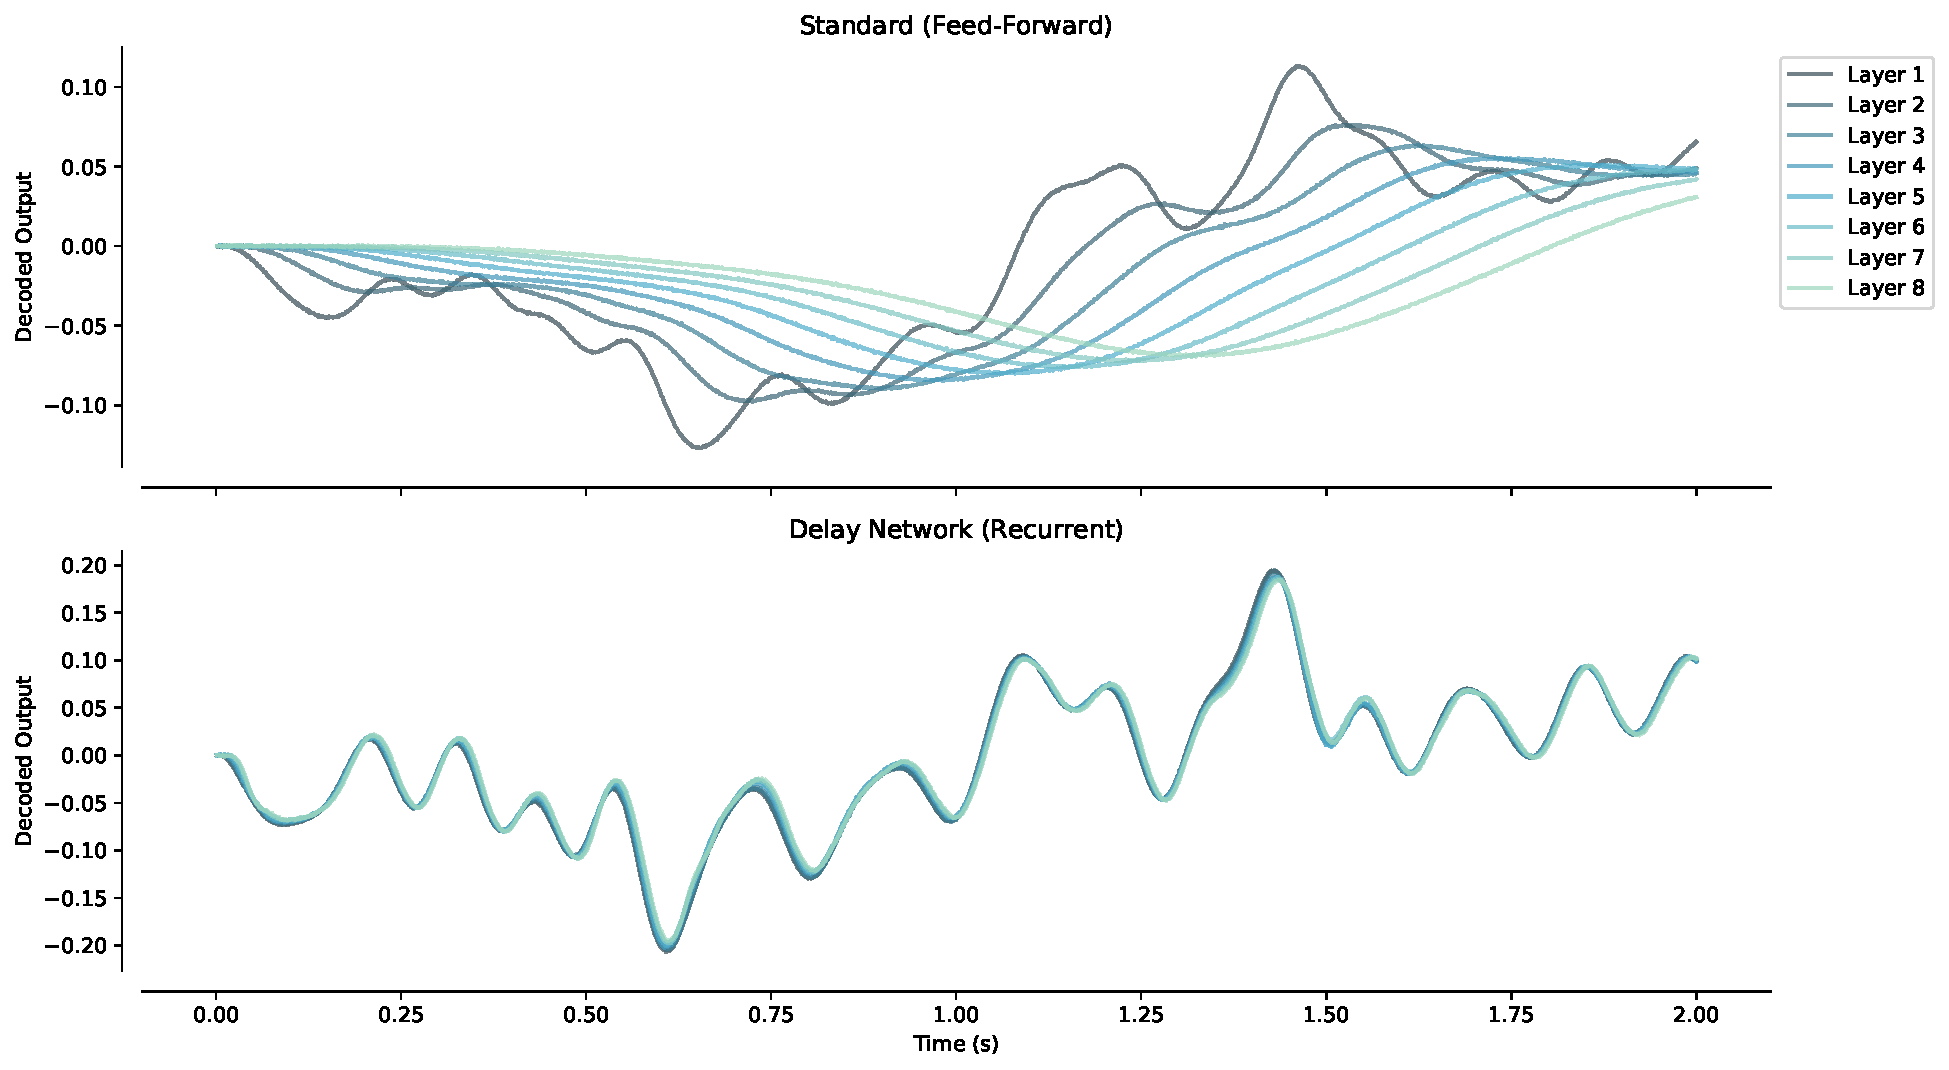
\includegraphics[width=\textwidth]{comm-channels}
     
    \caption{\label{fig:comm-channels} 
      Demonstrating the ability of the Delay Network~(DN) to approximate a synaptic deconvolution operation, realizing a pure communication channel.
      The test input $u(t)$ is a white noise signal band-limited at $10$\,Hz.
      (Top)~A standard feed-forward communication channel, implemented by decoding the identity function at each layer.
      (Bottom)~A recurrent communication channel, implemented by a Deep Delay Network~(DDN; section~\ref{sec:deep-delay-networks}) approximating $u(t)$ at each layer. Each layer is a NEF with $\theta = 50$\,ms and $q = 6$.
      In either case, there are $8$ layers of \numprint{2500} spiking LIF neurons, with each layer communicating spikes to the next through a lowpass synapse with time-constant $\tau = 100$\,ms.
    }
\end{figure}

\TODO{Demonstrate multiple layer communication channel without filtering.}

\subsection{Computing Taylor Series}
\label{sec:taylor-series}

\TODO{Linear map between state-vector and Taylor series of input signal expanded about any point.
More general than computing the derivative. Special case of a linear transformation of the input.}

\subsection{Computing Fourier Transform}
\label{sec:fourier-transform}

\TODO{Fourier Transform another special case of linear transformation}

\subsection{Detecting Repeating Patterns}
\label{sec:periodicity}

Given an arbitrary scalar signal, $u(t)$, we define a measure of \emph{$k$-periodicity} for natural $k \in \mathbb{N}_{\ge 1}$, with respect to some finite interval length $\theta > 0$, and sub-interval length $\gamma = \frac{\theta}{k}$, as follows:
\begin{equation} \label{eq:periodicity}
p_k(t) = \sqrt{ \frac{1}{\gamma} \int_{\tau=0}^{\gamma} \left( \frac{1}{k} \sum_{i=0}^{k-1} u \left( t - \theta + i \gamma + \tau \right) \right)^2 d\tau } \text{.}
\end{equation}
This can be computed directly by: (1) partitioning the last $\theta$ seconds into $k$ equally sized segments of length $\gamma$, (2) averaging them all together to obtain a superimposed signal of length $\gamma$, and (3) taking its root mean square (RMS).
When $p_k(t)$ is large relative to the overall RMS, this means that the $k$ segments constructively interfere and thus all segments contain approximately the same pattern. 
When $p_k(t)$ is maximal (i.e.,~equal to the RMS of the input signal), we refer to the signal  as being \emph{periodic}, since each of the $k$ segments must be exact copies of one another.
Lower values of $p_k(t)$ imply some amount of deconstructive interference within the superposition, and thus we refer to such signals as being \emph{aperiodic}.

We now present a method that can efficiently compute $p_k(t)$ with a SNN, by leveraging the computational properties of the Delay Network (DN).
This has applications as a general low-power signal processing tool, and for modelling how nontrivially-repeating patterns could be detected by neural mechanisms in a robust and flexible manner.

Our goal is to recast equation~\ref{eq:periodicity} to be in terms of the DN's state-vector, $\V{x}(t) \in \mathbb{R}^q$.
We claim that we may compute $p_k(t)$ by taking the L2-norm of the state-vector after a linear transformation:
\begin{align} \label{eq:approx-periodicity}
p_k(t) &\appropto \| P_k \V{x}(t) \| \\
P_k &= \frac{Z_k}{k} \sum_{i=0}^{k-1} e^{A i \gamma} \text{,} \label{eq:periodicity-matrix}
\end{align}
where $A$ is the recurrent state-space matrix from the balanced realization of equation~\ref{eq:ss-delay},\footnote{%
The proportionality $\propto$ in equation~\ref{eq:approx-periodicity} refers to a constant scaling in the balanced realization, while the approximation $\sim$ comes from the use of Pad\'e approximants to render the system finite-dimensional, and from assuming the DN mapping is unitary.
See text for details.
}
and $Z_k \in \mathbb{R}^{q \times q}$ is a ``zooming matrix'' computed by:
\begin{equation} \label{eq:zoom-matrix}
Z_k = B(0, 1)^+ B(1-1/k, 1) \text{,} % = \left( \transpose{B(0, 1)} B(0, 1) \right)^{-1} \transpose{B(0, 1)} B(1-1/k, 1) \text{,}
\end{equation}
where $(\cdot)^+$ denotes the Moore-Penrose pseudoinverse, $B(\cdot, \cdot) \in \mathbb{R}^{m \times q}$ is a matrix corresponding to a slice of the realized basis functions (equation~\ref{eq:basis-functions}), sampled along $m$ points, as in:
\begin{equation}
B(a, b) = \begin{pmatrix}
\mathcal{P}_{q-1,q}(a) & \cdots & \mathcal{P}_{0,q}(a) \\
\vdots & \vdots & \vdots \\
\mathcal{P}_{q-1,q}(b) & \cdots & \mathcal{P}_{0,q}(b)
\end{pmatrix} T \text{.}
\end{equation}
and $T$ is the similarity transform for the balanced realization.
A visualization of $Z_5$ is provided in Figure~\ref{fig:zoom-matrix}, using a diagonal $T$ to reveal its checkerboard structure.

\begin{figure}
  \centering
  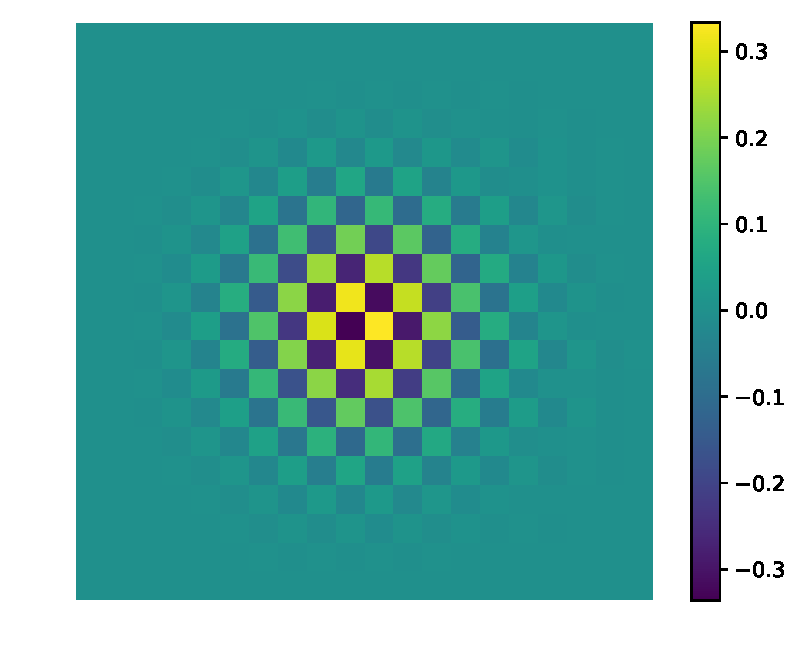
\includegraphics[width=0.4\textwidth]{zoom-matrix}
  \caption{\label{fig:zoom-matrix}
    Visualizing the ``zooming matrix'', $Z_k$ (see equation~\ref{eq:zoom-matrix}), for the case of $k=5$, $q=20$, $T$ taken by a digonal realization that normalizes the system's Hankel singular values, and the Moore-Penrose pseudoinverse taken while truncating the singular values below a cutoff ratio of 10\%.
   This matrix linearly transforms the state-space of the Delay Network to ``zoom in'' on the oldest segment of input history partitioned into $k$ segments.
  }
\end{figure}

We sketch a constructive proof of this claim.
Since the buffered window of input history is a linear transformation of the DN's state vector, we start by constructing a linear transformation of $\V{x}(t)$ that contains the average of all segments. 
The matrix $e^{A i \gamma}$ provides a linear transformation that emulates the effect of holding the input signal at zero for $i \gamma$ more seconds--a mathematical fast-forwarding of the system assuming no input.
This can be seen by solving the differential equation $\dot{\V{x}} = A \V{x}$ with the initial condition $\V{x}_0 = \V{x}(t)$.
Thus, $e^{A i \gamma} \V{x}(t)$ provides the state-vector that corresponds to some input signal where the $i^\text{th}$ segment (ordered by seniority) has been shifted back in time to become the oldest segment. 
Note that $e^0 = I$, and so the oldest segment ($i=0$) is not shifted.
More generally, $k^{-1} \left( I + e^{A \gamma} + \ldots + e^{A (k-1) \gamma} \right)$ linearly transforms the state-vector to correspond to an input signal where the oldest segment is the average of all segments.

Next, we must ``zoom in'' on the oldest segment.  
This zooming operation can be done by yet another linear transformation.
In particular, $Z_k$ is a linear transformation that takes us from a state-vector representing the entire interval of length $\theta$ to a state-vector representing the oldest sub-interval of length $\gamma$.
This is derived by observing that $B(1 - 1/k, 1)$ maps $\V{x}(t)$ onto the window of input history across the sub-interval $[t - \theta, t - \theta + \gamma]$---sampled along $m$ points---by construction.
Then $B(0, 1)^+$ reinterprets this sampled signal as a state-vector in the context of the full interval $[t - \theta, t]$.
To determine these matrices numerically, $m$ should be sufficiently large so as to approximate the limit as $m \rightarrow \infty$ within some tolerance.\footnote{%
We found $m = \numprint{1000}$ to be sufficient for our experiments.}

This same technique works without loss of generality to zoom in on any slice of the window, and reinterpret that segment of input as a new state-vector. This is a specific instantiation of the more general observation that the relationship between the state-vector and the input history is linear, and so any linear operation across the window (e.g., slicing, shifting, convolution, integral transforms, etc.) must also be linear with respect to the state-vector.
Moreover, by the scale-invariance of the delay network (see section~\ref{sec:delay-scalability}), all of the matrices (e.g., $Z_k$, $B(\cdot, \cdot)$, $P_k$) are independent of $\theta$. That is, these matrices only need to be precomputed once for some choice of $k$ and $q$, and applied to any $\theta$.

The last fact that we need is that the balanced realization is approximately unitary, in the sense that $\| \V{x}(t) \|$ is proportional to the RMS of its corresponding window of history.
\TODO{cite}
This conveniently implies that it sufficies to take the L2-norm of the resulting state-vector, as in equation~\ref{eq:approx-periodicity}, in order to obtain a proportional estimate of the RMS, $p_k(t)$, from equation~\ref{eq:periodicity}.
This completes our proof sketch.
To summarize, since the ideal computation involves a linear transformation of the input window, it can be recast as a linear transformation of the state.
And since the L2-norm of a balanced state reflects the RMS of its corresponding input signal, the former behaves as a proxy for the latter.

\begin{figure}
  \centering
  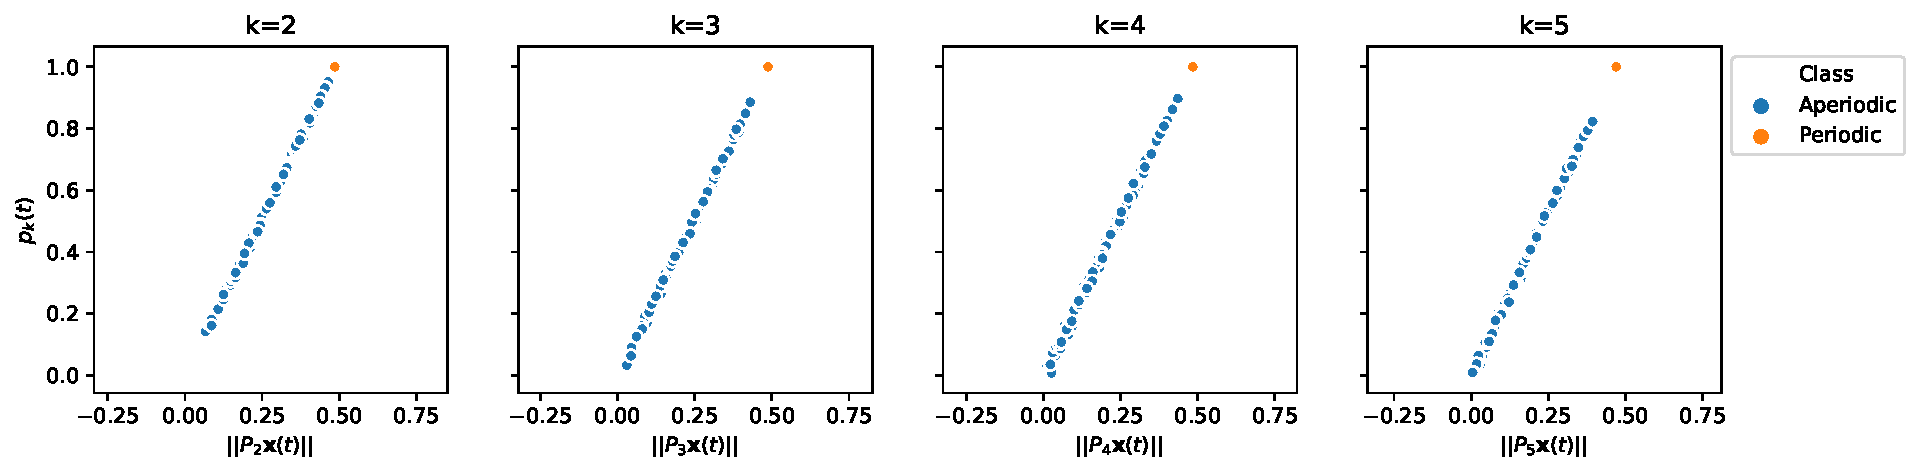
\includegraphics[width=1.0\textwidth]{periodicity}
  \caption{\label{fig:periodicity}
    The Delay Network (DN) approximating a measure of periodicity, tested against \numprint{1000} randomly generated input signals.
    The true measure of the input signal's $k$-periodicity, $p_k(t)$ (see equation~\ref{eq:periodicity}), is plotted on the $y$-axis, for two classes of input signals ($500$ periodic, and $500$ aperiodic), and $k \in \{2, 3, 4, 5\}$.
    The $x$-axis is the L2-norm of a linear transformation of the DN's state-vector, $\| P_k \V{x}(t) \|$ (see equation~\ref{eq:periodicity-matrix}).
    This empirically validates the claim of equation~\ref{eq:approx-periodicity} that the state-vector of the DN can be linearly transformed by a fixed matrix $P_k$ to proportionally-approximate a signal's $k$-periodicity.
  }
\end{figure}

We validate the above derivation by fixing $\theta=0.24$\,s, $q=20$, and then sampling white noise signals band-limited at $22$\,Hz (such that the error in the Pad\'e approximants, equation~\ref{eq:pade-delay-error}, is bounded above by 5\%) with RMS=$1$ from the two possible classes: periodic and aperiodic.
The periodic signals are generated by repeating a segment of length $\gamma$, $k$ times, while the aperiodic signals are random across the interval of length $\theta$.
In each case, the system of equations~\ref{eq:ss-delay} are balanced and simulated using zero-order hold~(ZOH) with a time-step of $\dt{} = 1$\,ms, to obtain the value of $\V{x}(t)$ at $t = \theta$.
The simulated value of $\| P_k(t) \|$ (equation~\ref{eq:periodicity-matrix}) is then compared to the ideal value of $p_k(t)$ (equation~\ref{eq:periodicity}).
The results in Figure~\ref{fig:periodicity} empirically validate the claim of equation~\ref{eq:approx-periodicity} for $k \in \{2, 3, 4, 5\}$, by demonstrating that $\|P_k \V{x}(t) \|$ proportionally-approximates the true $k$-periodicity.

Crucially, nothing has changed about the DN in order to support this brand of temporal pattern recognition.
The computation is merely a fixed linear transformation of the state, which is already being computed by the DN, followed by a nonlinear L2-norm operation.
Thus, in order to detect temporal patterns, computations such as measures of $k$-periodicity can be embedded as fixed linear transformations between the DN and additional pools of neural nonlinearities via Principles~1 and~2 of the NEF.

\subsection{Deep Delay Networks}
\label{sec:deep-delay-networks}

We now consider an architecture that stacks multiple DNs on top of one another, to form a \emph{Deep Delay Network}~(DDN) chaining multiple delays together.
For simplicity, we consider the case where each delay has the same length, $\gamma$, and each layer has the same dimensionality, $q$.
Thus, $k$ layers results in an overall delay of length $\theta = k \gamma$, and represents $k \cdot q$ total dimensions.

The state-vector of the $i^\text{th}$ layer, is denoted $\V{x}_i(t)$, where $i=0$ corresponds to the deepest layer (i.e., the last delay), and $i=k-1$ corresponds to the shallowest layer (i.e., the first delay).
We note that such an architecture realizes an alternative solution to computing the $k$-periodicity in section~\ref{sec:periodicity}; in particular, since $\V{x}_i(t)$ corresponds to the $i^\text{th}$ segment of input history, we have:
\begin{equation*}
P_k \V{x}(t) = \frac{1}{k} \sum_{i=0}^{k-1} \V{x}_i(t) \text{,}
\end{equation*}
where $P_k$ is the matrix defined by equation~\ref{eq:periodicity-matrix}, and $\V{x}(t)$ is the state-vector for an overall delay of length $\theta$.

We now determine the error in the overall delay by extending our analysis from section~\ref{sec:delay-scalability}.
Since each layer implements the transfer function $[q-1/q]e^{-\gamma s}$ (equation~\ref{eq:pade}), by the convolution theorem, the overall filter is the product of each transfer function.
Therefore, the error is characterized by the filter:
\begin{equation} \label{eq:deep-delay-network-error}
E_{q,k}(\theta s) = \left( [q-1/q]e^{-\gamma s} \right)^k - e^{-\theta s} \text{.}
\end{equation}
When $k = 1$, this reduces to equation~\ref{eq:pade-delay-error}.

\begin{figure}
  \centering
  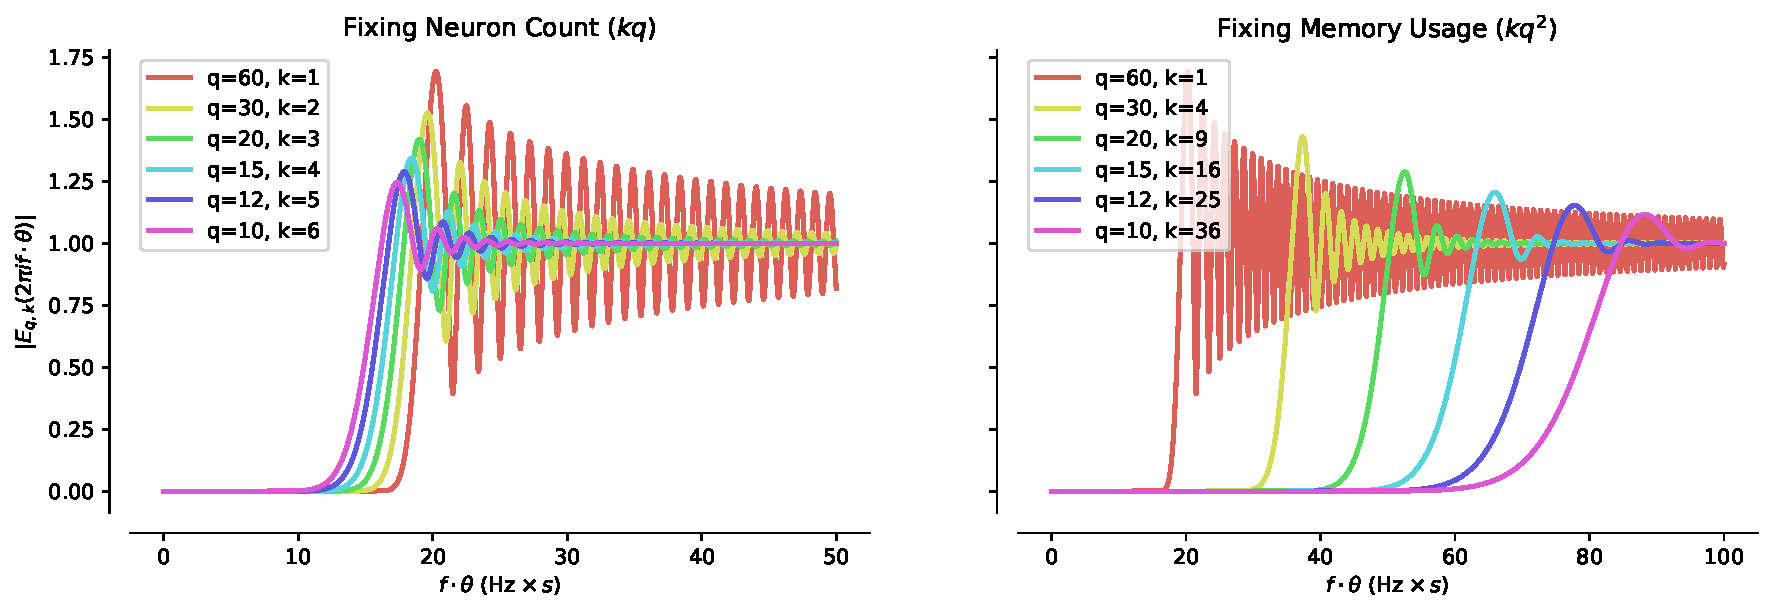
\includegraphics[width=1.0\textwidth]{deep-delay-network-error}
  \caption{\label{fig:deep-delay-network-error}
    Visualizing the error in the Deep Delay Network~(DDN) of width~$q$ and depth~$k$ (see equation~\ref{eq:deep-delay-network-error}) for two different resource-cost functions.
    (Left) Fixing the number of dimensions, $kq$, to be constant.
    Smaller $k$ scales further in this case.
    (Right) Fixing the density of connections, $kq^2$, to be constant.
    Smaller $q$ is more accurate in this case.
  }
\end{figure}

To gain insights into potential trade-offs between $k$ and $q$, we require additional constraints to keep the comparison meaningful.
If our main constraint is the number of neurons, then resource usage scales as $\bigoh{k q}$ given a constant level of accuracy per dimension.
However, if our main constraint is the number of multiply-adds and memory usage (i.e.,~connection density), then these scale as $\bigoh{k q^2}$ assuming the use of factored connection-weight matrices (as in the standard NEF formulation, and as realized on both SpiNNaker and Braindrop) and assuming the use of balanced state-space realizations.
In either case, we evaluate $E_{q,k}(\theta s)$ while varying $(q, k)$ to keep the resource-cost fixed (see Figure~\ref{fig:deep-delay-network-error}).

Depending on which resource-cost function is considered, we obtain very different trade-offs for the amount of error at some desired operating point $\theta s$ (see Figure~\ref{fig:pade-delay-error}).
In the former case of minimizing neural resources, we should set $k = 1$ and minimize $q$ such that $\theta s$ falls within the radius of convergence.
This should come as no surprise, as the DN has been derived to optimally approximate the delay line, and so there is no benefit to adding additional layers if we are free to scale $q$.
However, for the latter case of minimizing connectivity, we should primarily minimize $q$.
In other words, deeper structures provide an improvement in accuracy when paying $\bigoh{kq^2}$ for resources.

Furthermore, note that in Figure~\ref{fig:deep-delay-network-error}, the error oscillates with dampened amplitude beyond the radius of convergence for larger $k$.
This can be seen from equation~\ref{eq:deep-delay-network-error} by noticing that $[q-1/q]e^{-\gamma s}$ is a complex number with magnitude less than $1$, that is then exponentiated to the power of $k$.
By the same triangle-inequality argument in section~\ref{sec:delay-scalability}, this effectively regularizes the error $k$ times towards $1$ outside the radius of convergence.

The final consideration that should be made in picking $(q, k)$ is in determining the ideal nonlinear support for any function(s) to be computed across the window of history.
Since each dimension is encoded by a heterogeneous pool of neural nonlinearities, this supports the decoding of nonlinear functions with respect to the coefficient on the corresponding basis function (equation~\ref{eq:basis-functions}) via Principles~1 and~2.
Deeper networks effectively partition the basis functions into individual segments of input history, which enhances the complexity of the nonlinearities with respect to each segment, while limiting nonlinear interactions between segments.
All of this should be systematically taken into account when choosing the state-space realization, the delay lengths of each layer, the dimensionality of each layer, and the number of layers.

\subsection{Harnessing Higher-order Synapses}
\label{sec:pure_delay}

This section has been adapted from \citet{voelker2018}.

\TODO{Mention the existence of delays in Loihi and support of analog hardware such as in
``A programmable axonal propagation delay circuit for time-delay spiking neural networks''
Autoencoder in time.}

We begin by making the practical point that it is crucial to account for the effect of the simulation time-step in digital simulations, if the time-step is not sufficiently small relative to the time scale of the desired network-level dynamics.
To demonstrate this, we simulate a $27$-dimensional delay network using $\numprint{1000}$ spiking LIF neurons, implementing a $0.1$\,s delay of $50$\,Hz band-limited white noise.
We vary the simulation time-step ($\dt{}$) from $0.1$\,ms to $2$\,ms.
The accuracy of our extension does not depend on $\dt{}$ (see Figure~\ref{fig:principle3fail}(Left)).
When $\dt{}=1$\,ms (the default in Nengo), the standard Principle~3 mapping (equation~\ref{eq:p3-novel}) obtains a NRMSE of $1.425$ ($43\%$ worse than random chance), versus $0.387$ for the discrete lowpass mapping which accounts for $\dt{}$ (equation~\ref{eq:discrete-p3})---a $73\%$ reduction in error.
As $\dt{}$ approaches $0$ the two methods become equivalent.

More to the point, we can analyze the delay network's frequency response
%\footnote{%
%The frequency response is the transfer function evaluated at various input frequencies.
%}
when using a delayed continuous lowpass synapse (equation~\ref{eq:delayed-lowpass}) instead of the canonical lowpass (equation~\ref{eq:lowpass}) as the dynamical primitive.
This provides a direct measure of the possible improvement gains when using the extension.
Figure~\ref{fig:principle3fail}(Right) compares the use of Principle~3 (which accounts for $\tau$ but ignores $\lambda)$, to our extension (which fully accounts for both; see section~\ref{sec:delayed-lowpass}) when $\lambda = \tau$.
The figure reveals that increasing the dimensionality improves the accuracy of our extension, while magnifying the error from Principle~3.
In the worst case, the Principle~3 mapping has an absolute error of nearly $\numprint{e15}$.
In practice, saturation from the neuron model bounds this error by the maximum firing rates.
Regardless, it is clearly crucial to account for axonal transmission delays to accurately characterize the network-level dynamics.

\begin{figure}
  \centering
  \includegraphics[width=1.0\textwidth]{{NECO-04-17-2838-Figure.8}.pdf}
  \caption{\label{fig:principle3fail}
    Comparing standard Principle~3 to our NEF extensions.
    (Left)~Error from mapping a $27$-dimensional $0.1$\,s delay onto $\numprint{1000}$ spiking LIF neurons, while varying the simulation time-step ($\dt{}$).
    The input to the network is white noise with a cutoff frequency of $50$\,Hz.
    Unlike our extension, the standard form of Principle~3 does not account for $\dt{}$.
    A dashed vertical line indicates the default time-step in Nengo.
    Error bars indicate a $95\%$ confidence interval bootstrapped across $25$ trials.
    (Right)~Mapping the delay system onto a delayed continuous lowpass synapse (with parameters $\frac{\tau}{\theta} = 0.1$ and $\frac{\lambda}{\tau} = 1$).
    The order of the delay system ($q$) is varied from $6$ (lightest) to $27$ (darkest).
    Each line evaluates the error in the frequency response, $\left| e^{-\theta s} - F^H(H(s)^{-1}) \right|$, where $F^H$ is determined by mapping the delay of order $q$ onto equation~\ref{eq:delayed-lowpass} using one of the two following methods.
    The method of our extension---which accounts for the axonal transmission delay---has monotonically increasing error that stabilizes at $1$ (i.e.,~the high frequencies are filtered).
    The standard Principle~3---which accounts for $\tau$ but ignores $\lambda$---alternates between phases of instability and stability as the frequency is increased.
  }
\end{figure}

To more broadly validate our NEF extensions from section~\ref{sec:extensions}, we map the delay system onto:
(1)~a continuous lowpass synapse (see section~\ref{sec:lowpass});
(2)~a delayed continuous lowpass synapse (see section~\ref{sec:delayed-lowpass}); and
(3)~a continuous double-exponential synapse (see section~\ref{sec:general}).
We apply each extension to construct delay networks of $\numprint{2000}$ spiking LIF neurons.
To compare the accuracy of each mapping, we make the time-step sufficiently small ($\dt{} = 10\,\mu$s) to emulate a continuous-time setting.
We use the Pad\'e approximants of order $\left[5 / 6\right]$ for both equations~\ref{eq:pade} and~\ref{eq:lambert-delay}.
For the delayed lowpass, we again fix $\frac{\tau}{\theta} = 0.1$ and $\frac{\lambda}{\tau} = 1$.
For the double-exponential, we fix $\tau_1 = \tau$ and $\frac{\tau_1}{\tau_2} = 5$.
Expressing these parameters as dimensionless constants keeps our results scale-invariant with $\theta$.

\begin{figure}
  \centering
  \includegraphics[width=1.0\textwidth]{{NECO-04-17-2838-Figure.9}.pdf}
  \caption{\label{fig:lambert}
    The pure delay mapped onto spiking networks with various synapse models (with parameters $q = 6$, $\frac{\tau}{\theta} = 0.1$, $\frac{\lambda}{\tau} = 1$, $\tau_1 = \tau$, and $\frac{\tau_1}{\tau_2} = 5$).
    (Left)~Error of each mapping in the frequency domain.
    This subfigure is scale-invariant with $\theta$.
    (Right)~Example simulation when $\theta = 0.1\,$s and the input signal is white noise with a cutoff frequency of $15$\,Hz, corresponding to the triangle (over $1.5$) from the left subfigure.
    We use a time-step of $0.01$\,ms ($10\,\mu$s) and $\numprint{2000}$ spiking LIF neurons.
  }
\end{figure}

Figure~\ref{fig:lambert} reveals that axonal delays may be effectively ``amplified'' $10$-fold while reducing the NRMSE by $71\%$ compared to the lowpass (see Figure~\ref{fig:lambert}(Right); NRMSE for lowpass=$0.702$, delayed lowpass=$0.205$, and double-exponential=$0.541$).
The double-exponential synapse outperforms the lowpass, despite the additional poles introduced by the ZOH assumption in equation~\ref{eq:general-linear-approx} (see appendix~\ref{app:poles} for analysis).
This is because the double-exponential filters the spike-noise twice.
% Including the first-order derivative of the input signal further improves the double-exponential mapping by $X\%$.
Likewise, by exploiting an axonal delay, the same level of performance (e.g.,~$5\%$ error) may be achieved at approximately $1.5$ times higher frequencies, or equivalently for $1.5$ times longer network delays, when compared to the lowpass synapse (see~Figure~\ref{fig:lambert}(Left)).
In summary, accounting for higher-order synaptic properties allows us to harness the axonal transmission delay to more accurately approximate network-level delays in spiking dynamical networks.

Together, these results demonstrate that our extensions can significantly improve the accuracy of high-level network dynamics.
Having demonstrated this for delays, in particular, suggests that the extension is useful for a wide variety of biologically relevant networks (see section~\ref{sec:time-cells}).

Autocorelation (cosyne)
Storing and replaying episodic memories
Amplifying axonal spike delays
Amplifying one delay network into a larger delay network
